\documentclass[12pt,a4paper]{report}
\usepackage[utf8]{inputenc}
\usepackage[T1]{fontenc}
\usepackage[english]{babel}

\usepackage{geometry}
\usepackage{graphicx}
\usepackage{ulem}
\usepackage{amsmath}
\usepackage{amssymb,amsfonts,textcomp}
\usepackage{float}
\usepackage{listings}
\usepackage{algorithmic}
\usepackage{hhline}
\usepackage{array}
\usepackage{longtable}
\usepackage{fullpage}
\usepackage{supertabular}
\usepackage{hyperref}
\usepackage{fancyhdr}
\setlength{\headheight}{15.2pt}
\setlength{\headsep}{0.2in}

\newcounter{Figure}
\renewcommand\theFigure{\alph{Figure}}

\setcounter{secnumdepth}{4}
\setcounter{tocdepth}{4}

\lhead{Harry Milne}
\chead{Candidate Number: 2677}
\rhead{Centre Number: 22169}

\rfoot{\thepage}
\cfoot{}

\pagestyle{fancyplain}

\title{Home Face Authentication}
\author{Harry Milne}
\date{May 2014}

\lstset{
    language=Python,
    breaklines=true,
    numbers=left,
    frame=lines,
    showstringspaces=false
}


\begin{document}

\maketitle
\tableofcontents

\chapter{Analysis}
\section{Introduction}\label{section:_Toc370402491}
\subsection{Client Identification}\label{section:_Toc370402492}
The client is Paul Milne and this system will be for his household, the 
interest in developing this better system is purely for ease of use.

\subsection{Current System}\label{section:_Toc370402493}
The alarm system is for securing the house, there are alarms situated 
around the house on windows and doors which are wirelessly connected to 
the local network. The purpose for the alarm system is simply security.

Currently, to disable or enable the alarm a user must type in the set 
PIN into a number pad which is located near the stairs in the house. 
This is then sent to the server which controls all of the alarms in the 
house, the packet of data contains information which authenticates the 
device and the PIN which has been sent. If the PIN is correct, data is 
sent back to the number to give feedback stating the alarms have been 
now enabled or disabled. Otherwise it will reply with access denied and 
allow three more attempts before locking itself until a master password 
is inputted. 

\subsection{Problems}\label{section:_Toc370402494}
The main problem with the current system is that it is just too much 
hassle to keep track of a changing PIN and even to just enter it in 
twice a day. Replacing the current system with something that takes just 
a touch or even a look would save a lot of hassle with remembering PINs 
and setting them. This also leads onto the security itself of the PIN, 
it can easily be found on a piece of paper mistakenly thrown away which 
could give anyone access to the house.

\newpage
\subsection{Section Appendix}\label{section:_Toc370402495}
\textbf{Interview transcript:}
\lstinputlisting{initial_interview.log}

\section{Investigation}\label{section:_Toc370402496}
\subsection{The current system}\label{section:_Toc370402497}
\subsubsection{Data sources and destinations}\label{section:_Toc370402498}

\begin{table}[H]
\begin{tabular}{|l|p{4.5cm}|l|l|}
\hline
\textbf{Source} & \textbf{Data} & \textbf{Example Data} & \textbf{
Destination} \\
\hline
Client & Combination of Integers (length varying from 4 to 8 digits) & 
1234 & Numpad \\
\hline
Numpad & Packet containing combination and authentication data. & 
(\$auth\_info, "\,1234") & Server \\
\hline
Server & Packet containing success status and authentication data. & 
(\$auth\_info, True) & Numpad \\
\hline
Server & Packet containing authentication data and state that the device 
should be in. & (\$auth\_info, False) & Alarm \\
\hline
\end{tabular}
\end{table}
\newpage
\subsubsection{Algorithms}\label{section:_Toc370402499}
\paragraph{Number pad Process}

\begin{algorithmic}
\WHILE{true}
	\STATE $key\_entered\gets None$
	\STATE $pin\gets  ''$
	\WHILE{$key\_entered \neq stored\_pin$}
	    \STATE $pin\gets pin+key\_entered$
	\ENDWHILE
	\IF{$len(pin)\neq 4$}
	    \PRINT ERR: LENGTH
    \ELSE
        \STATE $server.send\_packet(pin)$
        \STATE $response\gets server.recv()$
        \IF{response}
            \PRINT GRANTED
        \ELSE
            \PRINT DENIED
        \ENDIF
    \ENDIF
\ENDWHILE
\end{algorithmic}

\paragraph{Server Process}

\begin{algorithmic}
\WHILE{true}
	\STATE $network.listen()$ \COMMENT{listen to packets being sent}
	\STATE $data\gets network.recv()$ \COMMENT{retrieve data from received packet}
	\IF{packet is valid}
	    \IF{user in database}
			\STATE $network.send(true)$ \COMMENT{send positive response back to device}
		\ELSE
			\STATE $network.send(false)$ \COMMENT{user did not match database}
		\ENDIF
	\ENDIF
\ENDWHILE

\end{algorithmic}

\subsubsection{Data flow diagram}\label{section:_Toc370402500}
\begin{figure}[H]

\includegraphics[scale=0.6]{media/image1.png}
\end{figure}


\begin{figure}[H]

\includegraphics[scale=0.6]{media/image2.png}
\end{figure}


\subsubsection{Input Forms, Output Forms, Report 
Formats}\label{section:_Toc370402501}
The only input to the current system is via the number pad to set and 
enter the PIN each time.

\subsection{The Proposed System}\label{section:_Toc370402502}
\subsubsection{Data sources and destinations}\label{section:_Toc370402503}

\begin{tabular}{|l|p{4.5cm}|l|l|}
\hline
\textbf{Source} & \textbf{Data} & \textbf{Example Data} & \textbf{
Destination} \\
\hline
Client & Face recognition data & This will be binary data. & Auth Device 
\\
\hline
Auth Device & Packet containing who the user is and the authentication 
data. & (\$auth\_info, "\,Paul") & Server \\
\hline
Server & Packet containing success status and authentication data. & 
(\$auth\_info, True) & Auth Device \\
\hline
Server & Packet containing authentication data and state that the device 
should be in. & (\$auth\_info, False) & Alarm \\
\hline
\end{tabular}


\subsubsection{Data flow diagram}\label{section:_Toc370402504}
\begin{figure}[H]

\includegraphics[width=15.92cm,height=4.28cm]{media/image3.eps}
\end{figure}


\begin{figure}[H]

\includegraphics[width=15.92cm,height=9.26cm]{media/image2.eps}
\end{figure}


\subsubsection{Data dictionary}\label{section:_Toc370402505}


\resizebox{15cm}{!}{
\begin{tabular}{|l|l|l|p{2.5cm}|p{2.5cm}|l|}
\hline
\textbf{Name} & \textbf{Type} & \textbf{Length} & \textbf{
Validation} & \textbf{Example Data} & \textbf{Comment} \\
\hline
UserID & Integer & 12 bit & N/A & 4095 & Unique to each user \\
\hline
UserName & String & 20 chars & Alphanumeric and $<$= 20 characters & 
"\,Paul" & Stored as tuple, first name index 0. \\
\hline
UserFaceData & Binary & N/A & N/A & N/A & Face recognition data. \\
\hline
EntryDate & String & 10 chars & N/A & "\,01/01/2013" & Generated when 
entry is validated. \\
\hline
Access\_Granted & Boolean & 1 bit & N/A & 1 & True if user was granted 
access. \\
\hline
Auth\_List & List & Variable & Valid IPs & 
("192.168.0.10",) & A list of saved authenticated 
devices \\
\hline
Auth\_Data & Binary & 1024-bit & N/A & (RSA Keys) & Used to check 
device's identity \\
\hline
\end{tabular}
}


\subsubsection{Volumetric}\label{section:_Toc370402506}
The size of the RAID that the database will be stored on is 4TB, this is 
populated with some other data but mostly is free space, so therefore 
the amount of logs or users will never feasibly reach over the size of 
the server's HDD because this is a home implementation of the system so 
there are minimal users.

\section{Objectives}\label{section:_Toc370402507}
\subsection{General Objectives}\label{section:_Toc370402508}
\begin{itemize}
\item Quick and easy to use method of user verification
\item Easy additional user setup
\item Communication with the server over the network
\item Store users and access logs in a SQL database
\end{itemize}
\subsection{Specific Objectives}\label{section:_Toc370402509}
\textbf{User Verification}

\begin{itemize}
\item Ability to recognize faces
\item Ability to tell different faces from others
\item Must be able to match a name to that face
\end{itemize}
\textbf{User Setup}

\begin{itemize}
\item UI to edit each user or add users
\item Power user tools
\end{itemize}
\textbf{Network Communication}

\begin{itemize}
\item Access to local area network
\item Receive commands and send commands
\item Secure
\end{itemize}
\textbf{SQL Database}

\begin{itemize}
\item Table containing each user
\item Access logs with a relationship to a user
\item Secure interface with communicating to the database
\end{itemize}
\subsection{Core Objectives}\label{section:_Toc370402510}
\begin{itemize}
\item User verification via face recognition
\item Interface with the server
\item Server to turn the alarms on and off
\end{itemize}
\subsection{Other Objectives}\label{section:_Toc370402511}
\begin{itemize}
\item Socket encryption
\item Control over what time slots people are allowed to turn alarms off
\item Ability to edit users from different computers
\end{itemize}
\section{E-R Diagrams and Descriptions}\label{section:_Toc370402512}
\subsection{E-R Diagram}\label{section:_Toc370402513}
\textbf{Database Relationships}

\begin{figure}[H]

\includegraphics[width=11.51cm,height=2.42cm]{media/image4.eps}
\end{figure}


\textbf{Hardware Relationship}

\begin{figure}[H]

\includegraphics[width=12.41cm,height=2.49cm]{media/image5.eps}
\end{figure}


\subsection{Entity Descriptions}%\label{section:_Toc370402514}

\textbf{User}(\underline{user\_no}, user\_name, face\_data) \newline
\textbf{Access}(\underline{access\_no}, date, \textit{user\_no})

\section{Object Analysis}\label{section:_Toc370402515}
\subsection{Object Listing}\label{section:_Toc370402516}
\begin{itemize}
\item AuthDevice
\begin{itemize}
\item Camera
\item NetworkInterface
\end{itemize}
\item Server
\begin{itemize}
\item SQLDatabase
\item NetworkInterface
\end{itemize}
\item Records
\begin{itemize}
\item UserRecord
\item AccessRecord
\end{itemize}
\end{itemize}



\subsection{Relationship diagrams}

\begin{figure}[H]
\includegraphics[width=15.92cm,height=9.99cm]{media/image6.eps}
\end{figure}


\subsection{Class Definitions}
\subsubsection{Client/AuthDevice}

Key

\begin{tabular}{|l|}
\hline
NAME \\
\hline
ATTRIBUTES \\
\hline
METHODS \\
\hline
\end{tabular}

Since this will be coded in Python methods aren't needed to 
retrieve attributes.



\begin{tabular}[h]{|l|}
\hline
\textbf{Camera} \\
\hline
active \\
\hline
resolution \\
\hline
face\_detected \\
\hline
change\_res \\
\hline
scan \\
\hline
log\_user \\
\hline
\end{tabular}


\begin{tabular}{|l|}
\hline
\textbf{NetworkInterface} \\
\hline
local\_address \\
\hline
master\_address \\
\hline
master\_port \\
\hline
update \\
\hline
auth \\
\hline
send\_record \\
\hline
recv\_record \\
\hline
\end{tabular}


\subsubsection{Server}\label{section:_Toc370402520}


\begin{tabular}{|l|}
\hline
\textbf{SQLDatabase} \\
\hline
size \\
\hline
number\_of\_users \\
\hline
number\_of\_records \\
\hline
search \\
\hline
add\_record \\
\hline
rm\_record \\
\hline
query \\
\hline
\end{tabular}


\begin{tabular}{|l|}
\hline
\textbf{NetworkInterface} \\
\hline
local\_address \\
\hline
local\_port \\
\hline
authed\_devices \\
\hline
auth \\
\hline
listen \\
\hline
reply \\
\hline
process \\
\hline
\end{tabular}


\subsubsection{Records}\label{section:_Toc370402521}


\begin{tabular}{|l|}
\hline
\textbf{UserRecord} \\
\hline
user\_no \\
\hline
user\_name \\
\hline
user\_facedata \\
\hline
\end{tabular}



\begin{tabular}{|l|}
\hline
\textbf{AccessRecord} \\
\hline
date \\
\hline
user \\
\hline
user\_no \\
\hline
\end{tabular}


\section{Other Abstractions}

\subsection{Graphs}\label{section:_Toc370402523}


\begin{figure}[h]
\includegraphics[width=15.92cm,height=8.97cm]{media/image7.eps}
\end{figure}


\section{Constraints}\label{section:_Toc370402524}
\subsection{Hardware}\label{section:_Toc370402525}
The budget allows the purchase of a Raspberry Pi and camera; this allows 
the project to be very flexible as there aren't many coding constraints. 
The server hardware will have no issue dealing with the amount of users 
(2) in a household, and logging the access of them.

This helps with development as it means I don't have restrictions in how 
I code or what libraries I choose to use meaning a lot more rapid 
development.

\subsection{Software}\label{section:_Toc370402526}
There are no constraints on what software to use other than the server's 
operating system being a Linux distribution, which doesn't really impact 
me since I won't have to install anything on the server apart from 
Python 3 and a SQL database, and they both work with all Linux 
distributions. 

This helps with development as it means I don't have restrictions in how 
I code or what libraries I choose to use meaning a lot more rapid 
development.

\subsection{Time}\label{section:_Toc370402527}
The deadline for the project is set by the college which is Monday the 
17$^{th}$ of February, 2014. The user has expressed no need for the 
system to be completed before this time.

\subsection{User Knowledge}\label{section:_Toc370402528}
The IT knowledge of this user is very high, so this means I will be able 
to explain exactly what I am implementing to him which just speeds up 
the process. This means I can implement the UI with efficiency of use in 
mind and because of his high IT proficiency he will be able to use it.

\subsection{Access restrictions}\label{section:_Toc370402529}
Admins will be able to access the data log and user management on the 
server; users will only be interacting with the mounted authentication 
device. This means I won't have to implement as much protection from 
accidental data deletion from users who don't know what they are doing; 
since they won't have access to it.

\section{Limitations}\label{section:_Toc370402530}
\subsection{Areas which will not be included in 
computerisation}\label{section:_Toc370402531}
\begin{itemize}
\item Other biometrics
\end{itemize}
Other biometrics such as finger print or retina recognition would 
improve the accuracy and security of this system but the hardware needed 
to implement this exceeds the client's budget.

\subsection{Areas considered for future 
computerisation}\label{section:_Toc370402532}
\begin{itemize}
\item Web interface/apps
\end{itemize}
Forms of modifying the system via either the Internet or other local 
devices while not being sat in front of the server or authentication 
device would be a good addition to the system; this allows for more user 
flexibility.



\section{Solutions}\label{section:_Toc370402533}
\subsection{Alternative solutions}\label{section:_Toc370402534}
\subsubsection{Face Recognition}\label{section:_Toc370402535}
Face recognition is a method of verification which allows no physical 
interaction from the user. This method of authentication has also been 
used by other companies such as Google's Android operating system, in 
which you glance or smile at your phone and it allows you access. This 
means there will already be plethora of documentation and information 
that can be found; this could help my development because it means a lot 
of testing has been done for me.

\subsubsection{Other biometrics}\label{section:_Toc370402536}
There are a few options with biometrics, including fingerprint, iris 
scanning, voice recognition; most of these methods are very much viable 
for user authentication but at an expense; they cost more. Most of these 
could be implemented into the future of the project because they add 
layers of security.

\subsubsection{NFC}\label{section:_Toc370402537}
The amount of devices capable of NFC (near field communication) has 
recently grown substantially, so this makes NFC a possible solution. 
However, this still isn't the majority of devices so a lot of users will 
not be able to use their personal devices for this method. Yet, if this 
system was being designed for a big company, they might distribute a 
company phone which could have this as one of its features, but the 
industry seems to be going in the opposite direction; the push is 
towards the use of personal devices for work.

\subsection{Justification of chosen solution}\label{section:_Toc370402538}
I decided to choose face recognition as the method of authentication 
because of the low budget and low costs of obtaining the equipment 
needed to use face recognition. All you require is a camera and the 
software will do the rest of the work. This method also detaches the 
user needing any kind of tech knowledge, all they need to do is look at 
the device and as soon as they are recognized they have done what they 
need to do; nothing complex to teach. 

\chapter{Design}

\section[Overall System Design]{Overall System Design}
\subsection[Short description of the main parts of the system]{Short description of the main parts of the system}

\begin{itemize}
\item Network House Alarm System with Biometric Authentication

\begin{itemize}
\item User Management
\item Face Recognition
\item Recording Access
\item Client/Server Network Communication
\end{itemize}
\end{itemize}
 \includegraphics[scale=0.4]{draftdesign-img/draftdesign-img1.png} 

\subsubsection[Overall Description]{Overall Description}
This system consists of two main parts, the master server, which deals with controlling the alarms around the house, and the authentication device (raspberry pi w/ video). The authentication device sends off a request over the network to deactivate or activate the alarm system when a face which matches the given face data is recognised, the master server then checks this user against its own database and logs the state change of the system. The device receives a packet back from the master stating the current state to give feedback to the user. 

\subsubsection[User Management]{User Management}
The system administrator needs to be able to edit the users within the system’s database easily, therefore a UI or a CLI must be coded giving an interface to the database.

\subsubsection[Face Recognition]{Face Recognition}
The device that takes face input needs to be triggered when the user wants their face recognised to toggle the alarm system, this requires some form of physical button or signal to the device so that it knows to start searching for a face to verify.

\subsubsection[Recording Access]{Recording Access}
When a user is authenticated the time and date with the user ID needs to be saved to a database; this allows the system administrator to review when users have accessed the building.

\subsubsection[Client/Server Network Communication]{Client/Server Network Communication}
The server which is the centre of the system needs to be able to communicate with all the devices across the local area network so that the face recognition can be verified and the alarms can be activated when the authentication is successful.

\subsection[System flowcharts showing an overview of the complete system]{System flowcharts showing an overview of the complete system}
\subsubsection[Main System Loop]{Main System Loop}
{\centering  \includegraphics[scale=0.4]{draftdesign-img/draftdesign-img2.png} \par}

\subsubsection[Camera Process]{Camera Process}
{\centering  \includegraphics[scale=0.4]{draftdesign-img/draftdesign-img3.png} \par}

{\centering
The camera uses a generated XML file which contains the face data of the users who want to be recognized.
\par}

\section[User Interface Designs]{User Interface Designs}
\subsection[Database Management Table Tabs]{Database Management Table Tabs}
The tabs shown in the wireframe below give quick and easy access to the data inside the database, to edit any of these fields is also just a doubleclick.

{\centering  \includegraphics{draftdesign-img/draftdesign-img4.png} \par}

{\centering  \includegraphics{draftdesign-img/draftdesign-img5.png} \par}

{\centering  \includegraphics{draftdesign-img/draftdesign-img6.png} \par}

\subsection[Database Management Menu Bar]{Database Management Menu Bar}
I have thought about the kind of features I’d want in a database interface, such as exporting and finding. These should cover most database usage.

{\centering  \includegraphics{draftdesign-img/draftdesign-img7.png} \par}

{\centering
 \includegraphics{draftdesign-img/draftdesign-img8.png}  
\par}

{\centering
Here the user creation requires an input, so a dialog will popup, however the Log File creation does not, so it will just display information in the status bar.
\par}

{\centering
\  \includegraphics{draftdesign-img/draftdesign-img9.png} 
\par}

{\centering  \includegraphics{draftdesign-img/draftdesign-img10.png} \par}

{\centering
The menu selections above simply open a file browser dialog where you choose where to save the file.
\par}

\subsection[Find Dialogs]{Find Dialogs}
{\centering  \includegraphics{draftdesign-img/draftdesign-img11.png} \par}

Below you can enter a search criteria to look through all relevant tables, after you have the results you can also export this data into a txt or csv file using the default Windows file browser.

{\centering  \includegraphics{draftdesign-img/draftdesign-img12.png}  \includegraphics{draftdesign-img/draftdesign-img13.png} \par}

\section[Hardware Specification]{Hardware Specification}
The master server requires a PC with a VDU and network connection so that the admin can access the database management tool and the server can reach the authentication device.
This system requires a programmable device which has video and network compatibility, in this case I have chosen to use a Raspberry Pi. This gives me the most flexibility to select whatever software’s I need at a low price, it will be running on a distribution of Debian with 512MB of RAM, the low hardware specifications for this device limits the frame rate at which I can process video from the camera, however this isn’t an issue because a high enough frame rate can be reached to make the program functional. I am also using the Logitech C270 because of its cheap price and compatibility with not only the raspberry pi but OpenCV.

\section[Program Structure]{Program Structure}
\subsection[Top down design structure charts]{Top down design structure charts}

\includegraphics[scale=0.5]{draftdesign-img/draftdesign-img14.png}

\includegraphics[scale=0.5]{draftdesign-img/draftdesign-img15.png}

\subsubsection[Key]{Key}


\begin{tabular}{| m{8cm} | m{8cm} |}
\hline
\bfseries Variable Names &
\bfseries Description\\\hline
\bfseries t/f & 
Boolean\\\hline
\bfseries i & 
image\\\hline
\bfseries u &
User \(string\)\\\hline
\bfseries d &
data\\\hline
\bfseries pd &
Packet data\\\hline
\bfseries r &
Response\\\hline
\end{tabular}


\bigskip

\subsection[Algorithms in pseudo{}-code for each data transformation process]{Algorithms in pseudo-code for each data transformation process}


\begin{tabular}{|m{2.569cm}|m{9.944cm}|m{3.188cm}|}
\hline
Function &
Pseudo-code &
Description\\\hline
user\_certainty &
FUNCTION user\_certainty (Faces: Array)

\ \ \_CERTAINTY\_THRESHOLD: Integer

\ \ \_CERTAINTY\_THRESHOLD {\textless}- 7 //highest is 10, lowest is 1

\ \ passed\_faces: Array* //init dynamic array for faces that pass

\ \ face\_array\_length {\textless}- length(Faces);

\ \ FOR i {\textless}- 1 TO face\_array\_length

\ \ \ \ IF Faces[i].certainty {\textgreater} 7

\ \ \ \ \ \ passed\_faces[length(passed\_faces)+1] {\textless}- Faces[i] //append to pass\_faces

\ \ RETURN passed\_faces

ENDFUNCTION &
Checks detected objects and returns satisfying detections.\\\hline
construct\_packet &
FUNCTION construct\_packet (Username: String)

\ \ packet\_data: String

\ \ packet\_data {\textless}- {\textquotedbl}REQUEST {\textquotedbl}+Username;

\ \ network.send\_packet(packet\_data.encode());

ENDFUNCTION &
Takes username and appends command then encodes and sends\\\hline
parse\_packet &
FUNCTION parse\_packet (data\_r: String)

\ \ command, user: String

\ \ arg\_list: Array

\ \ arg\_list {\textless}- data\_r.split({\textquotedbl} {\textquotedbl}); //split string into array where whitespace

\ \ IF arg\_list[0] == {\textquotedbl}REQUEST{\textquotedbl}

\ \ \ \ command {\textless}- arg\_list[0]

\ \ \ \ user {\textless}- arg\_list[1]

\ \ IF arg\_list[0] == {\textquotedbl}STUFF{\textquotedbl}

\ \ \ \ command {\textless}- arg\_list[0]

\ \ \ \ stuff {\textless}- arg\_list[1]

\ \ RETURN \{{\textquotedbl}command{\textquotedbl}:command, {\textquotedbl}user{\textquotedbl}:user, {\textquotedbl}stuff{\textquotedbl}:stuff\} //returning dict

ENDFUNCTION &
Splits received strings into an argument list\\\hline
~
 &
~
 &
~
\\\hline
\end{tabular}



\subsection[Object diagrams]{Object diagrams}
 \includegraphics[scale=0.5]{draftdesign-img/draftdesign-img16.png} 

\subsection[initions]{initions}

\textit{Key}


\begin{tabular}{|l|}
\hline
NAME\\\hline
ATTRIBUTES\\\hline
METHODS\\\hline
\end{tabular}

\subsubsection[Client]{Client}

\begin{tabular}{|l|}
\hline
\textbf{Camera}\\\hline
active\\
resolution\\
face\_detected\\\hline
change\_res\\
scan\\
log\_user\\\hline
\end{tabular}
\begin{tabular}{|l|}
\hline
\textbf{NetworkInterface}\\\hline
local\_address\\
master\_address\\
master\_port\\\hline
update\\
auth\\
send\_record\\
recv\_record\\\hline
\end{tabular}

\subsubsection[Server]{Server}


\begin{tabular}{|l|}
\hline
\textbf{SQLDatabase}\\\hline
size\\
number\_of\_users\\
number\_of\_records\\\hline
search\\
add\_record\\
rm\_record\\
query\\\hline
\end{tabular}
\begin{tabular}{|l|}
\hline
\textbf{NetworkInterface}\\\hline
local\_address\\
local\_port\\
authed\_devices\\\hline
auth\\
listen\\
reply\\
process\\\hline
\end{tabular}

\subsubsection[Records]{Records}

\begin{tabular}{|l|}
\hline
\textbf{User}\\\hline
user\_no\\
user\_name\\
user\_facedata\\\hline
\end{tabular}
\begin{tabular}{|l|}
\hline
\textbf{Record}\\\hline
date\\
user\\
user\_no\\\hline
\end{tabular}



\section[Prototyping]{Prototyping}
\subsection[Consideration of impact on design and development]{Consideration of impact on design and development}
The main part of the system that will need a prototype created is the face recognition on the raspberry pi, I will need to set up an environment where I can easily debug and test the camera input. This requires me to attach the raspberry pi to a monitor so I get visual feedback. This helps me to work out kinks in which the feature recognition software may act unexpectedly, without much of a way to view the console it’d be very hard to find out what actually went wrong and how I can fix it.

Other things that I would consider to create prototypes would include:

\begin{itemize}
\item The encryption of sockets needs to be tested and prototyped so I have a stronger idea of how to implement this. After prototyping this I can also be more certain in the way it works and also be quicker in debugging because I can test the scenario on the prototype.
\item Authentication of a device, I need to be able to make sure I can securely authenticate each device. Otherwise intruders on the network may be able to mimic a client and receive data. This is important because the whole point of this system is that it’s for security, finding out ways in which intruders may gain access will help me secure the system.
\end{itemize}


\section[Definition of Data Requirements]{Definition of Data Requirements}
\subsection[Identification of all data input items]{Identification of all data input items}
\begin{itemize}
\item User names
\item Face data for recognition
\end{itemize}
\subsection[Identification of all data output items]{Identification of all data output items}
\begin{itemize}
\item Log file containing logs of user interaction
\item Text/CSV files from SQL Queries
\item Signals to alarms around house
\item TCP packets to either side of the system.
\end{itemize}
\subsection[Explanation of how data output items are generated]{Explanation of how data output items are generated}
The log file is generated over time as the system is used, each interaction with the system will be logged on a new line of the log file.

\subsection[Data Dictionary]{Data Dictionary}


\resizebox{15cm}{!}{
\begin{tabular}{|m{2.516cm}|m{2.472cm}|m{2.476cm}|m{2.578cm}|m{2.552cm}|m{2.506cm}|}
\hline
\textbf{Name} &
\textbf{Data Type} &
\textbf{Length} &
\textbf{Validation} &
\textbf{Example Data} &
\textbf{Comment}\\\hline
UserID &
Integer &
12 bit &
N/A &
4095 &
Unique to each user\\\hline
UserName &
String &
20 chars &
Alphanumeric and {\textless}= 20 characters &
“Paul” &
Stored as tuple, first name index 0.\\\hline
UserFaceData &
Binary &
N/A &
N/A &
N/A &
Face recognition data.\\\hline
EntryDate &
String &
10 chars &
N/A &
“01/01/2013” &
Generated when entry is validated.\\\hline
Access\_Granted &
Boolean &
1 bit &
N/A &
1 &
True if user was granted access.\\\hline
Auth\_List &
List &
Variable &
Valid IPs &
[“192.168.0.10”,

“192.168.0.11”) &
A list of saved authenticated devices\\\hline
Public\_Key &
Long &
1024-bit &
N/A &
N/A &
Public key used in the current system.\\\hline
Log\_Filename &
string &
20 chars &
N/A &
Entry.log &
Used to identify the current log file in use\\\hline
Private\_key &
long &
1024-bit &
N/A &
N/A &
Used as a private encryption variable.\\\hline
\end{tabular}
}


\bigskip

\subsection[Identification of appropriate storage media]{Identification of appropriate storage media}
The raspberry pi runs all on an SD card, which is more than enough to handle the OS, modules required and face data. There is no other way for the raspberry pi to operate so I am limited to using this SD card, however I see no downsides to it and no reason to implement any other form of storage.

You would only need a USB Flash Drive to back up the data stored in a SQL database and a log file, since both are very small files, the master server itself will have a HDD to store everything on so size of the database is not a concern.

\section[Database Design]{Database Design}
\subsection[Normalisation]{Normalisation}
\subsubsection[ER Diagrams]{ER Diagrams}
\includegraphics[scale=0.5]{draftdesign-img/draftdesign-img17.png}


\subsubsection[UNF to 3NF]{UNF to 3NF}


\begin{tabular}{|l|l|l|l|l|l|l|}
\hline
UNF &
~
 &
1NF &
~
 &
2NF &
~
 &
3NF\\\hline
user\_name &
* &
user\_id &
* &
user\_id &
* &
user\_id\\\hline
user\_id &
~
 &
user\_name &
~
 &
user\_name &
~
 &
user\_name\\\hline
record\_date &
~
 &
~
 &
~
 &
~
 &
~
 &
~
\\\hline
record\_id &
* &
record\_id &
* &
record\_id &
* &
record\_id\\\hline
record\_toggle &
* &
\textit{user\_id} &
~
 &
\textit{user\_id} &
~
 &
\textit{user\_id}\\\hline
log\_id &
~
 &
record\_date &
~
 &
record\_date &
~
 &
\textit{log id}\\\hline
log\_filen &
~
 &
record\_toggle &
~
 &
record\_toggle &
~
 &
record\_date\\\hline
log\_created &
~
 &
log\_created &
~
 &
log\_id &
~
 &
record\_toggle\\\hline
~
 &
~
 &
log\_filen &
~
 &
log\_filen &
~
 &
~
\\\hline
~
 &
~
 &
log\_id &
~
 &
log\_created &
* &
log\_id\\\hline
~
 &
~
 &
~
 &
~
 &
~
 &
~
 &
log\_filen\\\hline
~
 &
~
 &
~
 &
~
 &
~
 &
~
 &
log\_created\\\hline
\end{tabular}

Primary key = *

\subsection[SQL Queries]{SQL Queries}
\subsubsection[User]{User}


\resizebox{15cm}{!}{
\begin{tabular}{|m{7.951cm}|m{7.9490004cm}|}
\hline
\bfseries SQL Query &
\bfseries Description\\\hline
insert into Users(user\_name) values (?) &
Adds a user to the database\\\hline
delete from Users where user\_id = ? &
Delete user with certain id\\\hline
select * from Users &
Lists all columns and rows from table ‘Users’\\\hline
select * from Users where user\_name = ? &
Select all columns where user name is a certain value\\\hline
select user\_name from Users where user\_id = ? &
Select user name from user id\\\hline
\end{tabular}
}

\subsubsection[Logs]{Logs}

\resizebox{15cm}{!}{
\begin{tabular}{|m{7.951cm}|m{7.9490004cm}|}
\hline
\bfseries SQL Query &
\bfseries Description\\\hline
insert into Log(log\_filen, log\_created) values (?,?) &
Create a new log row in table ‘Log’\\\hline
select * from Log where log\_id=(SELECT MAX(log\_id) FROM Log) &
Returns latest Log file information\\\hline
\end{tabular}
}

\subsubsection[Access]{Access}

\resizebox{15cm}{!}{
\begin{tabular}{|m{7.951cm}|m{7.9490004cm}|}
\hline
\bfseries SQL Query &
\bfseries Description\\\hline
insert into Access(user\_id, log\_id, access\_date, access\_toggle) values (?,?,?,?) &
Create new Access row in table ‘Access’\\\hline
select * from Access where user\_id = ? &
Get all access’s from ‘Access’ which have the user id = ?\\\hline
\end{tabular}
}


\bigskip

\section[Security and Integrity of the System and Data]{Security and Integrity of the System and Data}
\subsection[Security and Integrity of Data]{Security and Integrity of Data}
Keeping the communication between the parts of this system secure is very important; this is because if any intruder manages to trick the system into thinking it is a authenticated client then the intruder can access and send requests to the server.

I will be keeping communication secure by using the Diffie-Hellman key exchange to make sure the server to client know they are speaking to each other. This will be implemented alongside a keyword which the device will need to authenticate with the server. If the keyword is wrong, the device will be ignored.

\subsection[System Security]{System Security}
There are two levels of access, system administrator and user. The user only has access to toggling the alarm system, whereas the system administrator deals with database management. The system needs to be physically at the server to do any of the work, so this is already protected by the operating system installed on the server.

\section[Validation]{Validation}

\resizebox{15cm}{!}{
\begin{tabular}{|m{5.2310004cm}|m{5.235cm}|m{5.2380004cm}|}
\hline
\bfseries Variable &
\bfseries Validation Rule &
\bfseries eg\\\hline
\bfseries username &
No non-alpha characters &
ACCEPT: Harry DECLINE: !h4rry\\\hline
\bfseries Datetime &
Meet the format DD/MM/YYYY HH:MM &
ACCEPT: 17/01/2014 00:00 DECLINE: 17.01.14 00,00\\\hline
\bfseries Search term &
No non-alpha characters &
ACCEPT: Harry DECLINE: !h4rry\\\hline
\end{tabular}
}


\bigskip

\section[Testing]{Testing}
\subsection[Outline Plan]{Outline Plan}
\subsubsection[Identification and explanation of suitable test strategies]{Identification and explanation of suitable test strategies}

\resizebox{15cm}{!}{
\begin{tabular}{|m{3.8749998cm}|m{3.8749998cm}|m{3.873cm}|m{3.878cm}|}
\hline
\bfseries Test Series &
\bfseries Purpose &
\bfseries Testing Strategy &
\bfseries Strategy Rationale\\\hline
\bfseries 1 &
Testing of individual functions/objects &
Unit testing &
Ensuring each function returns and operates correctly leads to easier testing of the system as a whole\\\hline
\bfseries 2 &
Test that the separately developed systems work together e.g client and server &
Integration testing &
For any system-wide testing to commence, this is a must.\\\hline
\bfseries 3 &
Test that the system works to the minimal function intended &
Black box testing &
Later in the development process it is important to test that the modules are actually working at least to some extent.\\\hline
\bfseries 4 &
Thorough testing of data flow between each object &
White box testing &
Accounts for every possibility that could happen within this system\\\hline
\bfseries 5 &
Testing in real world scenarios &
Alpha testing &
Before users should interact with a version of this system, a real world test should be performed in-house.\\\hline
\bfseries 6 &
Customer satisfaction &
Acceptance testing &
To ensure the user is happy with the finished product is of utmost impoortance\\\hline
\end{tabular}
}


\bigskip


\bigskip


\bigskip


\bigskip

\subsection[Detailed Plan]{Detailed Plan}

\begin{longtable}{|l|m{2.375cm}|m{2.682cm}|m{1.416cm}|m{2.238cm}|m{1.181cm}|m{1.8369999cm}|}
\hline
\bfseries No. &
\bfseries Purpose &
\bfseries Description &
\bfseries Test Data Type &
\bfseries Expected Result &
\bfseries Actual Result &
\bfseries Evidence \\\hline
\bfseries 1.1 &
SQLite3 DB API &
Testing of each function within the database API is important because of how central this is to the system. &
String &
Correct data from the database. &
~
 &
~
\\\hline
\bfseries 1.2 &
Face scanning function &
Testing of the function that scans an image for a face. &
Feature object array &
Non-empty list when correct face in image &
~
 &
~
\\\hline
\bfseries 1.3 &
Network communication functions &
Sending packets and commands between the server and the client. &
String /

Network &
Receiving a string when one is sent &
~
 &
~
\\\hline
\bfseries 1.4 &
System loops &
Testing of each function which starts a system loop. &
Runtime &
Loop starts without errors &
~
 &
~
\\\hline
\bfseries 1.5 &
Individual faces function &
Testing to make sure individuals faces are picked up and not everyone’s. &
N/A &
Face/feature objects created only when given faces are in frame &
~
 &
~
\\\hline
\bfseries 2.1 &
Face scanning with Network communication &
Test that when a face is recognised it triggers a network packet and listens for a response. &
N/A &
Packets sent and received from the master server. &
~
 &
~
\\\hline
\bfseries 2.2 &
DB API with Client requests &
Test that the database is modified correctly when connected with the client device. &
Sqlite &
Access logged, log file created. &
~
 &
~
\\\hline
\bfseries 2.3 &
House alarms with master server signals &
Triggering the house alarms from the master server &
Network &
Alarms are disabled and enables appropriately &
~
 &
~
\\\hline
\bfseries 2.4 &
Network response triggers LEDs on raspberry pi &
Response from the master server triggers the LEDs to on or off. &
Network &
Red LED turns on when access is denied, Green LED turned on when access is granted &
~
 &
~
\\\hline
\bfseries 3.1 &
Minimal function test &
Test that the system works so that users can disable/enable the house alarms. &
N/A &
Face recognition to trigger a state change on the server and alarms. &
~
 &
~
\\\hline
\bfseries 4.1 &
Test the intended way through the system (almost 3.1) &
Routing through the main functions &
N/A &
No errors &
~
 &
~
\\\hline
\bfseries 4.2 &
Test with faces that don’t match data on the raspberry pi &
Routing through functions that handle faces not fitting the data &
N/A &
No access granted &
~
 &
~
\\\hline
\bfseries 4.3 &
Time test &
Leave the system running without interaction to test stability &
N/A &
No crashing &
~
 &
~
\\\hline
\bfseries 4.4 &
~
 &
~
 &
~
 &
~
 &
~
 &
~
\\\hline
\bfseries 5.1 &
Test the system over a day with constant use &
This is the test how the system with react to sustained use. &
Runtime &
Stability &
~
 &
~
\\\hline
\bfseries 6.1 &
Allow the user to spend time using and testing the prototype itself &
This makes sure that the client is happy with how the project is turning out &
N/A &
Satisfaction &
~
 &
~
\\\hline
\bfseries 6.2 &
Later customer test &
Allow the user to test the system nearer to the end of its development cycle. &
N/A &
Satisfaction &
~
 &
~
\\\hline
\end{longtable}

\chapter{Testing}

\section{Test Plan}
\subsection{Detailed Test Plan}
The shaded areas have been changed from the original plan from the 

\tablehead{}
\begin{supertabular}{|m{2.259cm}|m{2.375cm}|m{3.936cm}|m{1.416cm}|m{4.6860003cm}|}
\hline
\bfseries Test Series and number &
\bfseries Purpose &
\bfseries Description &
\bfseries Test Data Type &
\bfseries Expected Result\\\hline
\bfseries 1.1 &
SQLite3 DB API &
Testing of each function within the database API is important because of how central this is to the system. &
String &
Correct data from the database.\\\hline
\bfseries 1.2 &
Face scanning function &
Testing of the function that scans an image for a face. &
Feature object array &
Non-empty list when correct face in image\\\hline
\bfseries 1.3 &
Network communication functions &
Sending packets and commands between the server and the client. &
String /

Network &
Receiving a string when one is sent\\\hline
\bfseries 1.4 &
System loops &
Testing of each function which starts a system loop. &
Runtime &
Loop starts without errors\\\hline
\bfseries 1.5 &
Individual faces function &
Testing to make sure individuals faces are picked up and not everyone’s. &
N/A &
Face/feature objects created only when given faces are in frame\\\hline
\bfseries 2.1 &
Face scanning with Network communication &
Test that when a face is recognised it triggers a network packet and listens for a response. &
N/A &
Packets sent and received from the master server.\\\hline
\bfseries 2.2 &
DB API with Client requests &
Test that the database is modified correctly when connected with the client device. &
Sqlite &
Access logged, log file created.\\\hline
\bfseries 2.3 (REMOVED) &
House alarms with master server signals &
Triggering the house alarms from the master server &
Network &
Alarms are disabled and enables appropriately\\\hline
\bfseries 2.4 (REMOVED) &
Network response triggers LEDs on raspberry pi &
Response from the master server triggers the LEDs to on or off. &
Network &
Red LED turns on when access is denied, Green LED turned on when access is granted\\\hline
\bfseries 3.1 &
Minimal function test &
Test that the system works so that users can disable/enable the house alarms. &
N/A &
Face recognition to trigger a state change on the server and alarms.\\\hline
\bfseries 4.1 &
Test the intended way through the system (almost 3.1) &
Routing through the main functions &
N/A &
No errors\\\hline
\bfseries 4.2 &
Test with faces that don’t match data on the raspberry pi &
Routing through functions that handle faces not fitting the data &
N/A &
No access granted\\\hline
\bfseries 4.3 (REMOVED) &
Time test &
Leave the system running without interaction to test stability &
N/A &
No crashing\\\hline
\bfseries 5.1 (REMOVED) &
Test the system over a day with constant use &
This is the test how the system with react to sustained use. &
Runtime &
Stability\\\hline
\bfseries 6.1 (MODIFIED) &
Test all menus &
Test all of the available menus in the menu bar &
N/A &
No errors and actions ran\\\hline
\bfseries 6.11 &
Test status bar &
Check that text appears when entities are created in the database &
N/A &
~
\\\hline
\bfseries 6.2 (MODIFIED) &
Test combo box &
Test that the widget performs as expected &
N/A &
Modified view of the widget\\\hline
\bfseries 6.3 (NEW) &
Test editing values &
Test editing values with the tables generated in the Database Browser. &
String &
Changes commit and persist after closing of UI\\\hline
\bfseries 6.4 (NEW) &
Test all menus (without database opened) &
Test all of the available menus in the menu bar &
N/A &
Inappropriate actions disabled.\\\hline
\bfseries 6.5 (NEW) &
Test combo box (without database opened) &
Test that the widget performs as expected &
N/A &
Inappropriate actions disabled.\\\hline
\end{supertabular}


\bigskip

\subsection{Changes from original plan}
Originally the plan had acceptance testing (6.*) from the user, instead I have replaced that with the user interface testing which was not previously part of the detailed test plan. I did this because of the time restrictions in place by my teacher. The tests 2.4 and 4.3 have both been removed also due to time limits.

\section{Test Data}
\subsection{Test Data}
\subsubsection{Normal Test Data used for Test Series 1.1}

\tablehead{}
\begin{supertabular}{|m{5.097cm}|m{5.099cm}|m{5.1060004cm}|}
\hline
\textbf{Function Name} &
\textbf{Test Data Example} &
\textbf{Expected Result}\\\hline
\_\_init\_\_ &
“access.sqlite3” &
No return value\\\hline
init\_log &
No parameters &
Folders created\\\hline
create\_tables &
No parameters &
Tables created\\\hline
add\_user &
“helloworld” &
User “helloworld” created\\\hline
rm\_user &
1 &
User with ID of 1 deleted\\\hline
ls\_users &
No parameters &
A list of users names in the database\\\hline
fetch\_user\_id &
“helloworld” &
Return the ID of user with the name “helloworld”\\\hline
fetch\_username &
1 &
Return the username of the user with an ID of 1\\\hline
create\_log\_file &
No parameters &
Create a blank log file and database entry\\\hline
get\_latest\_log &
No parameters &
Return the latest log file entity\\\hline
append\_latest\_log &
“a message” &
Append a message to the latest log\\\hline
log\_access &
log\_access(“helloworld”, True) &
Log a state change in the alarm appropriately\\\hline
logs\_by\_user &
1 &
Return all of the logs made by the user with an ID of 1\\\hline
\end{supertabular}

\subsubsection{Erroneous Test Data used for Test Series 1.1}

\tablehead{}
\begin{supertabular}{|m{5.097cm}|m{5.099cm}|m{5.1060004cm}|}
\hline
\textbf{Function Name} &
\textbf{Test Data Example} &
\textbf{Expected Result}\\\hline
\_\_init\_\_ &
“sadas” &
Throw missing file error\\\hline
init\_log &
No parameters &
Folders created\\\hline
create\_tables &
No parameters &
Tables created\\\hline
add\_user &
@\$\%\^{}\&*wdf &
User “@\$\%\^{}\&*wdf” created\\\hline
rm\_user &
821378174 &
SQLite3 error, User doesn’t exist.\\\hline
ls\_users &
No parameters &
A list of users names in the database\\\hline
fetch\_user\_id &
“\$6sd7\%\^{}\&” &
SQLite3 error, User doesn’t exist.\\\hline
fetch\_username &
12137 &
SQLite3 error, User doesn’t exist.\\\hline
create\_log\_file &
No parameters &
Create a blank log file and database entry\\\hline
get\_latest\_log &
No parameters &
Return the latest log file entity\\\hline
append\_latest\_log &
“no erroneous data available for a string” &
Append a message to the latest log\\\hline
log\_access &
log\_access(“helworld”, “test”)

log\_access(“helworld”, 1)

log\_access(123, 0) &
Throw error\\\hline
logs\_by\_user &
121314 &
SQLite3 error, User doesn’t exist.\\\hline
\end{supertabular}


\bigskip

\subsection{Changes from original data}
\section{Annotated Samples}
\subsection{Actual Results}
\subsubsection[Normal Data for Test Series 1.1]{Normal Data for Test Series 1.1}
\label{bkm:Ref381956334}
\tablehead{}
\begin{supertabular}{|m{4.04cm}|m{6.1610003cm}|m{5.102cm}|}
\hline
\textbf{Function Name} &
\textbf{Test Data Example} &
\textbf{Actual Result}\\\hline
\_\_init\_\_ &
“access.sqlite3” &
{\textgreater}{\textgreater}{\textgreater} s = SQLInterface({\textquotedbl}access.sqlite3{\textquotedbl})

logs/access/

An unexpected print statement shows something needs to be modified about the functions that run in \_\_init\_\_\\\hline
init\_log &
No parameters &
{\textgreater}{\textgreater}{\textgreater} s.init\_log()

logs/access/

The result from this test gives me the function that was causing the previous unexpected stdout.\\\hline
create\_tables &
No parameters &
Figure 3.2.1 a \\\hline
add\_user &
“helloworld” &
Figure 3.2.1 b\\\hline
rm\_user &
1 &
Figure 3.2.1 c\\\hline
ls\_users &
No parameters &
Empty database gives:

{\textgreater}{\textgreater}{\textgreater} s.ls\_users()

[]

Populated database gives:

{\textgreater}{\textgreater}{\textgreater} sql.ls\_users()

[u{\textquotesingle}harry{\textquotesingle}, u{\textquotesingle}paul{\textquotesingle}, u{\textquotesingle}alyson{\textquotesingle}, u{\textquotesingle}jane{\textquotesingle}, u{\textquotesingle}ava{\textquotesingle}]

{\textgreater}{\textgreater}{\textgreater}\\\hline
fetch\_user\_id &
“helloworld” &
{\textgreater}{\textgreater}{\textgreater} s.fetch\_user\_id({\textquotedbl}helloworld{\textquotedbl})

1

{\textgreater}{\textgreater}{\textgreater}

This returned the correct user ID, as shown in Figure 3.2.1 a.\\\hline
fetch\_username &
1 &
{\textgreater}{\textgreater}{\textgreater} s.fetch\_username(1)

u{\textquotesingle}helloworld{\textquotesingle}

{\textgreater}{\textgreater}{\textgreater}

This returned the correct username, as shown in Figure 3.2.1 a.\\\hline
create\_log\_file &
No parameters &
Log file created as shown in Figure 3.2.1 d\\\hline
get\_latest\_log &
No parameters &
{\textgreater}{\textgreater}{\textgreater} sql.get\_latest\_log()

(4, u{\textquotesingle}14-03-06T234247.log{\textquotesingle}, u{\textquotesingle}14-03-06T234247{\textquotesingle})

{\textgreater}{\textgreater}{\textgreater}\\\hline
append\_latest\_log &
“a message” &
Figure 3.2.1 e\\\hline
log\_access &
log\_access(“helloworld”, True) &
Figure 3.2.1 f\\\hline
logs\_by\_user &
1 &
{\textgreater}{\textgreater}{\textgreater} sql.logs\_by\_user(1)

[(1, 1, 1, u{\textquotesingle}14-03-06T22:31:13{\textquotesingle}, 1), (2, 1, 1, u{\textquotesingle}14-03-06T22:32:25{\textquotesingle}, 0), (3, 1, 1, u{\textquotesingle}14-03-06T22:32:25{\textquotesingle}, 1), (4, 1, 1, u{\textquotesingle}14-03-06T22:32:28{\textquotesingle}, 0), (5, 1, 1, u{\textquotesingle}14-03-06T22:56:06{\textquotesingle}, 1), (6, 1, 1, u{\textquotesingle}14-03-06T22:56:54{\textquotesingle}, 0), (7, 1, 1, u{\textquotesingle}14-03-06T23:00:40{\textquotesingle}, 1), (8, 1, 1, u{\textquotesingle}14-03-06T23:08:18{\textquotesingle}, 0)]

{\textgreater}{\textgreater}{\textgreater}\\\hline
\end{supertabular}

\subsubsection[Erroneous Data for Test Series 1.1]{Erroneous Data for Test Series 1.1}
\label{bkm:Ref381956364}
\tablehead{}
\begin{supertabular}{|m{4.04cm}|m{6.1610003cm}|m{5.102cm}|}
\hline
\textbf{Function Name} &
\textbf{Test Data Example} &
\textbf{Actual Result}\\\hline
\_\_init\_\_ &
“sadas” &
Database file called “sadas” created.\\\hline
add\_user &
@\$\%\^{}\&*wdf &
Figure 3.2.1 g\\\hline
rm\_user &
821378174 &
No exception, ran without error.\\\hline
fetch\_user\_id &
“\$6sd7\%\^{}\&” &
{\textgreater}{\textgreater}{\textgreater} ed.fetch\_user\_id({\textquotedbl}\$6sd7\%\^{}\&{\textquotedbl})

Traceback (most recent call last):

\ \ File {\textquotedbl}{\textless}stdin{\textgreater}{\textquotedbl}, line 1, in {\textless}module{\textgreater}

\ \ File {\textquotedbl}sql\_interface.py{\textquotedbl}, line 83, in fetch\_user\_id

\ \ \ \ result = self.db\_cursor.fetchone()[0]

TypeError: {\textquotesingle}NoneType{\textquotesingle} object has no attribute {\textquotesingle}\_\_getitem\_\_{\textquotesingle}

{\textgreater}{\textgreater}{\textgreater}\\\hline
fetch\_username &
12137 &
{\textgreater}{\textgreater}{\textgreater} ed.fetch\_username(12137)

Traceback (most recent call last):

\ \ File {\textquotedbl}{\textless}stdin{\textgreater}{\textquotedbl}, line 1, in {\textless}module{\textgreater}

\ \ File {\textquotedbl}sql\_interface.py{\textquotedbl}, line 90, in fetch\_username

\ \ \ \ return self.db\_cursor.fetchone()[0]

TypeError: {\textquotesingle}NoneType{\textquotesingle} object has no attribute {\textquotesingle}\_\_getitem\_\_{\textquotesingle}

{\textgreater}{\textgreater}{\textgreater}\\\hline
log\_access &
log\_access(“helworld”, “test”)

log\_access(“helworld”, 1)

log\_access(123, 0) &
{\textgreater}{\textgreater}{\textgreater} ed.log\_access({\textquotedbl}helworld{\textquotedbl}, {\textquotedbl}test{\textquotedbl})

Traceback (most recent call last):

\ \ File {\textquotedbl}{\textless}stdin{\textgreater}{\textquotedbl}, line 1, in {\textless}module{\textgreater}

\ \ File {\textquotedbl}sql\_interface.py{\textquotedbl}, line 114, in log\_access

\ \ \ \ user\_id = self.fetch\_user\_id(user\_name)

\ \ File {\textquotedbl}sql\_interface.py{\textquotedbl}, line 83, in fetch\_user\_id

\ \ \ \ result = self.db\_cursor.fetchone()[0]

TypeError: {\textquotesingle}NoneType{\textquotesingle} object has no attribute {\textquotesingle}\_\_getitem\_\_{\textquotesingle}

{\textgreater}{\textgreater}{\textgreater}\\\hline
logs\_by\_user &
121314 &
{\textgreater}{\textgreater}{\textgreater} ed.logs\_by\_user(121314)

[]

{\textgreater}{\textgreater}{\textgreater}\\\hline
\end{supertabular}


\bigskip

\subsubsection{Test Plan Results}

\tablehead{}
\begin{supertabular}{|m{2.257cm}|m{2.8339999cm}|m{3.2979999cm}|m{2.0509999cm}|m{4.464cm}|}
\hline
\bfseries Test Series and number &
\bfseries Purpose &
\bfseries Description &
\bfseries Test Data Type &
\bfseries Actual Result\\\hline
\bfseries 1.1 &
SQLite3 DB API &
Testing of each function within the database API is important because of how central this is to the system. &
String &
Shown at Normal Data for Test Series 1.1 and Erroneous Data for Test Series 1.1\\\hline
\bfseries 1.2 &
Face scanning function &
Testing of the function that scans an image for a face. &
Feature object array &
SimpleCV.Features.Detection.HaarFeature at (320,252)\\\hline
\bfseries 1.3 &
Network communication functions &
Sending packets and commands between the server and the client. &
String /

Network &
Figure 3.2.2 h\\\hline
\bfseries 1.4 &
System loops &
Testing of each function which starts a system loop. &
Runtime &
Example of client loop starting:

Figure 3.2.3 i

Example of server loop starting:

Figure 3.2.3 j\\\hline
\bfseries 1.5 &
Individual faces function &
Testing to make sure individuals faces are picked up and not everyone’s. &
N/A &
The check\_face function only returns one face, even when multiple are in the image. The most prominent will be returned.\\\hline
\bfseries 2.1 &
Face scanning with Network communication &
Test that when a face is recognised it triggers a network packet and listens for a response. &
N/A &
Works as shown in Figure 3.2.4 k.\\\hline
\bfseries 2.2 &
DB API with Client requests &
Test that the database is modified correctly when connected with the client device. &
Sqlite &
Figure 3.2.5 l shows how the database and log file have been created and updated correctly.\\\hline
\bfseries 2.3 &
House alarms with master server signals &
Triggering the house alarms from the master server &
Network &
The state of the server changes when the according state is sent from the client. 

: INFO \ \ \ \ harry recognised

: INFO \ \ \ \ state toggled to True\\\hline
\bfseries 2.4 (REMOVED) &
Network response triggers LEDs on raspberry pi &
Response from the master server triggers the LEDs to on or off. &
Network &
Red LED turns on when access is denied, Green LED turned on when access is granted\\\hline
\bfseries 3.1 &
Minimal function test &
Test that the system works so that users can disable/enable the house alarms. &
N/A &
Face recognition to trigger a state change on the server and alarms.\\\hline
\bfseries 4.1 &
Test the intended way through the system (almost 3.1) &
Routing through the main functions &
N/A &
No errors\\\hline
\bfseries 4.2 &
Test with faces that don’t match data on the raspberry pi &
Routing through functions that handle faces not fitting the data &
N/A &
The system correctly matches faces with given data.\\\hline
\bfseries 4.3 (REMOVED) &
Time test &
Leave the system running without interaction to test stability &
N/A &
No crashing\\\hline
\bfseries 5.1 (REMOVED) &
Test the system over a day with constant use &
This is the test how the system with react to sustained use. &
Runtime &
Stability\\\hline
\bfseries 6.1 (MODIFIED) &
Test all menus &
Test all of the available menus in the menu bar &
N/A &
Shown in Test Series 6.1\\\hline
\bfseries 6.11 (NEW) &
Test status bar &
Check that text appears when entities are created in the database &
N/A &
Text correctly appears in the status bar, as shown in Test Series 6..\\\hline
\bfseries 6.2 (MODIFIED) &
Test combo box &
Test that the widget performs as expected &
N/A &
Combo box correctly switches between tables of the database.\\\hline
\bfseries 6.3 (NEW) &
Test editing values &
~
 &
~
 &
Works as shown in Test Series 6.3\\\hline
\bfseries 6.4 (NEW) &
Test all menus (without database opened) &
Test all of the available menus in the menu bar &
N/A &
Appropriate menus disabled. Test Series 6.4 \\\hline
\bfseries 6.5 (NEW) &
Test combo box (without database opened) &
Test that the widget performs as expected &
N/A &
Appropriately disabled. Test Series 6.5\\\hline
\end{supertabular}


\bigskip


\bigskip


\bigskip


\bigskip


\bigskip


\bigskip


\bigskip


\bigskip


\bigskip


\bigskip


\bigskip


\bigskip


\bigskip


\bigskip


\bigskip


\bigskip


\bigskip

\subsection{Evidence}
\subsubsection[Test Series 1.1]{Test Series 1.1}
\label{bkm:Ref381981653}
\bigskip


\includegraphics[scale=0.5]{media/testdraft-img1.png}
 

\label{bkm:Ref381949304}Figure 3.2.1\stepcounter{Figure}{\theFigure}

The above shows that the tables were created successfully in the given database file.


\bigskip

 
\includegraphics[scale=0.5]{media/testdraft-img2.png}
 

\label{bkm:Ref381949457}Figure 3.2.1\stepcounter{Figure}{\theFigure}

A user was created with a user\_name of “helloworld” and ID of 1.

 
\includegraphics[scale=0.5]{media/testdraft-img3.png}
 

\label{bkm:Ref381949913}Figure 3.2.1\stepcounter{Figure}{\theFigure}

This shows the change from Figure 3.2.1 b, the user as now been deleted.


\bigskip

 
\includegraphics[scale=0.3]{media/testdraft-img4.png}
 

\label{bkm:Ref381952028}Figure 3.2.1\stepcounter{Figure}{\theFigure}


\bigskip

 
\includegraphics[scale=0.3]{media/testdraft-img5.png}
 

\label{bkm:Ref381952713}Figure 3.2.1\stepcounter{Figure}{\theFigure}


\bigskip

 
\includegraphics[scale=0.5]{media/testdraft-img6.png}
 

\label{bkm:Ref381953001}Figure 3.2.1\stepcounter{Figure}{\theFigure}

Shown above is the function “log\_access” being run and adding to a log file.


\bigskip

 
\includegraphics[scale=0.5]{media/testdraft-img7.png}
 

\label{bkm:Ref381955967}Figure 3.2.1\stepcounter{Figure}{\theFigure}

\subsubsection{Test Series 1.3}

\bigskip

 
\includegraphics[scale=0.5]{media/testdraft-img8.png}
 

\label{bkm:Ref381956602}Figure 3.2.2\stepcounter{Figure}{\theFigure}

Here you can see data being received from the client, no errors occur while testing these functions.

\subsubsection{Test Series 1.4}

\bigskip

 
\includegraphics[scale=0.4]{media/testdraft-img9.png}
 

\label{bkm:Ref381959717}Figure 3.2.3\stepcounter{Figure}{\theFigure}

In Figure 3.2.3 i you can see the client loop starting and starting to scan for faces that match the stored “harry.jpg”.


\bigskip

 
\includegraphics[scale=0.5]{media/testdraft-img10.png}
 

\label{bkm:Ref381959735}Figure 3.2.3\stepcounter{Figure}{\theFigure}

\subsubsection{Test Series 2.1}

\bigskip


\bigskip

 
\includegraphics[scale=0.5]{media/testdraft-img11.png}
 

\label{bkm:Ref381964963}Figure 3.2.4\stepcounter{Figure}{\theFigure}

In Figure 3.2.4 k you can see the server on the top and the client at the bottom, the client text shows that a ‘HaarFeature’ has been found and has matched the stored image. This process is shown in the server by the line saying that “harry” has been recognised.

\subsubsection{Test Series 2.2}
 
\includegraphics[scale=0.3]{media/testdraft-img12.png}
 

\label{bkm:Ref381970622}Figure 3.2.5\stepcounter{Figure}{\theFigure}

Both the database and log file updated correctly.

\subsubsection[Test Series 6.1]{Test Series 6.1}
\label{bkm:Ref381978952}
\bigskip

 
\includegraphics[scale=0.5]{media/testdraft-img13.png}
 

\label{bkm:Ref381976684}Figure 3.2.6\stepcounter{Figure}{\theFigure}

Clicking “User” in Figure 3.2.6 mFigure 3.2.4 k leads to Figure 3.2.6 n, this is the intended action. Clicking “Log File”, sucessfully creates a new entity in the “Log” table. Refresh Database reloads the widget displaying the data and Load Database shows the dialog in Figure 3.2.5 l.

 
\includegraphics[scale=0.5]{media/testdraft-img14.png}
 

\label{bkm:Ref381976679}Figure 3.2.6\stepcounter{Figure}{\theFigure}

 
\includegraphics[scale=0.4]{media/testdraft-img15.png}
 

Figure 3.2.6\stepcounter{Figure}{\theFigure}

\subsubsection[Test Series 6.11]{Test Series 6.11}
\label{bkm:Ref381979575} 
\includegraphics[scale=0.5]{media/testdraft-img16.png}
 

Figure 3.2.7\stepcounter{Figure}{\theFigure}


\bigskip

 
\includegraphics[scale=0.5]{media/testdraft-img17.png}
 

Figure 3.2.7\stepcounter{Figure}{\theFigure}

\subsubsection[Test Series 6.3]{Test Series 6.3}
\label{bkm:Ref381981093}
\bigskip

 
\includegraphics[scale=0.5]{media/testdraft-img18.png}
 

\label{bkm:Ref381980635}Figure 3.2.8\stepcounter{Figure}{\theFigure}

As shown in Figure 3.2.8 r, I have edited and reopened the database from the user interface. The changes successfully saved and displayed correctly, as shown in Figure 3.2.8 s.

 
\includegraphics[scale=0.5]{media/testdraft-img19.png}
 

\label{bkm:Ref381980687}Figure 3.2.8\stepcounter{Figure}{\theFigure}


\subsubsection[Test Series 6.4]{Test Series 6.4}
\label{bkm:Ref381981128}
\bigskip

 
\includegraphics[scale=0.5]{media/testdraft-img20.png}
 

Figure 3.2.9\stepcounter{Figure}{\theFigure}

\subsubsection[Test Series 6.5]{Test Series 6.5}
\label{bkm:Ref381981150} 
\includegraphics[scale=0.7]{media/testdraft-img21.png}
 

Figure 3.2.10\stepcounter{Figure}{\theFigure}


\bigskip

\section[Evaluation]{Evaluation}
\subsection{Approach to testing}
Firstly my approach was to carefully unit test the real backbone of the code, the SQL interface, for example in Test Series 1.1 I took each function and checked the outputs. As the program gets bigger it’s a lot harder to individually test the different components, so I moved to black-box testing for most of the rest of the testing. Knowing that my SQL code was up to standard and respond with accurate results meant that I could pinpoint bugs a lot quicker than if I wasn’t sure if the interface to the database was solid.

\subsection{Problems}
Testing only really unveiled a few slight bugs, mainly just remnants of previous bug testing, for example print statements that had been left in. My main issue with the code in its current state is that it lacks polish, this is wholly down to time constraints that I thought weren’t much of an issue to begin with. However, as development continued, problems which weren’t so easy to fix arose. This severely decreased the amount of time I actually had to code and increased battle with pre-existing code. 

\subsection{Strengths}
Strengths of my testing was making sure that the functions which the entire project relies on, the database interface, was robust. This ensured that obscure errors didn’t occur with the handled data. 

\subsection{Weaknesses}
The weaknesses of my testing would be the detail, I would like to go a lot more in-depth into each function and ensure they are all polished, however time does not allow this. Black-box testing is sufficient for getting out a product that works but not so well at making sure you aren’t wasting computing resources with unnecessary code.

\subsection{Reliability}
It is hard to test how reliable my implementation of face recognition is, simply because of the number of ways you can exploit it. For instance, holding a picture up in front of the camera would suffice as a match to the stored images. Another variable that is introduced is light levels, you can get very different results from cameras if you take pictures in different light levels, therefore the program will struggle to find the matches in the images. I have combatted this by not taking one picture but taking a live feed until a match has been found, yet it still isn’t definite a match will occur.

\subsection{Robustness}
With the time I have had running the code, it all seems very robust. Three different components working together could have meant that they wouldn’t be very robust but I haven’t managed to make the system crash. However this is helped along by the lack of human error introduced to this program, so therefore it doesn’t need to account for it.

\chapter{System Maintenance}

\section{Environment}
    \label{sec:env}
    \subsection{Software}
    \begin{itemize}
        \item Python 2.7 and included modules
        
        \begin{itemize}
            \item SQLite3
        \end{itemize}
        
        \item Twisted 13.2.0 Python Module
        \item PyQt4 Python Module
        \item SimpleCV 1.3
        \item SQLite Database Browser
        \item Vim
        \item Sublime Text 3
    \end{itemize}

    \begin{table}[H]
        \centering
        \begin{tabular}{|p{4cm}|p{8cm}|}
        \hline
        \textbf{Software}                & \textbf{Usage Explanation}                                                                                                                                                                                            \\ \hline
        Python 2.7              & I used Python 2.7 instead of Python 3.* because of the superior module support that Python 2.5+ has. Also, the nature of Python itself makes it very easy to build systems quickly.                          \\ \hline
        SQLite3                 & SQLite3 was an easy database management system to use because it has little requirements for the system it is run on. This means you do not have to do any extensive configuration of any target system.      \\ \hline
        Twisted 13.2.0          & Twisted is a Python module which lets you very quickly prototype and build clients and servers, which is central to this system.                                                                             \\ \hline
        PyQt4                   & PyQt4 is a feature rich user interface development module, it handles all of the threading needed to run operations while keeping an operational interface.                                                  \\ \hline
        SimpleCV 1.3            & SimpleCV is aimed at making computer vision easy to develop, I used it in conjunction with the Raspberry Pi to recognise faces.                                                                              \\ \hline
        SQLite Database Browser & This open source software gives an easy way to visually check over your SQLite databases, this was invaluable in testing.                                                                                    \\ \hline
        Vim                     & When developing the python server script, it was easier to program it while on the server itself instead of deploying to it every time I wanted to test. This meant using a text editor that works in shell. \\ \hline
        Sublime Text 3          & This was the editor of choice while programming in a GUI environment, it has a lot of tools to help with syntax highlighting and variable naming.                                                            \\ \hline
        \end{tabular}
    \end{table}


\section{System Overview}
The system has 3 main components; the client, server and database browser. The server and client are directly related
whereas the database browser is a `tool' I have bundled to help the user manage the database. The database browser works
with the server on a local level, in that you edit the same file on the same system that the server does. However,
the database browser requires the server to be running a graphical user environment because it is a graphical representation
of the database. 

    \subsection{Client}
    The client uses the SimpleCV package as shown in section~\ref{sec:env}, this package handles everything around the camera,
    this makes it easier to read what is happening with the data being handled by the Python. The client package needs to be
    running everywhere where you want to be able to toggle the alarm system. 

    \subsection{Server}
    The server will be installed on a dedicated computer which will not be turned off, the Python script runs as a daemon
    which the Twisted Python package (section~\ref{sec:env})) handles. The server can be set up to use whatever port is defined
    in the configuration file, as mentioned in section~\ref{sec:settings}, this should be the exact same number as every client
    uses.

    The server needs to be running for the client to interact with the alarm system, otherwise the client will receive network
    errors.

    \subsection{Database Browser}
    The database browser gives the system administrator an easy interface to edit the database, this is required for
    adding new users to the system. Once the client and server are set up with the same users the system will work
    correctly. Unfortunately there was no easy way to set up the system to update every single node whenever a user is
    added, so this tool is necessary for the system to work.


\section{Code Structure}
I structured the code so that each section of the system was an object, abstracting like this helps a lot with
visualising the code. By doing this I have taken one of the advantage of object-oriented programming; the ability
to abstract certain situations into particular `objects'.

    \subsection{Client Class}
    \label{sec:clientstructure}
    The class created in `client.py', which can be found in section~\ref{sec:client.py}, includes methods to handle
    the processing of images that it will be continuously scanning. 

    The code is laid out so that the face recognition methods and networking methods are physically separated, this means
    coming back to file file isn't a lot of scrolling trying to find the appropriate functions, instead they are somewhat
    ordered.

    The most prominent method in the `Client' class is the `start' method, this triggers the client to start processing
    images from the given camera. This loop is purposely infinite because it is a daemon and doesn't need to `finish', unlike
    most conventional code where the code has an `end' state, this just loops until a `KeyboardInterrupt' is triggered.

    \lstinputlisting[language=Python, 
                    firstline=36, 
                    lastline=47,
                    label={lst:clientstart},
                    caption=The start method from section~\ref{sec:client.py}.]{code/client/client.py}

    \subsection{Handler Class}
    The server class created in `server.py' is called `Handler' as shown in section~\ref{sec:server.py} line 8, this is 
    because it `handles' the requests from the client. Inside this class there is an `SQLInterface' instantiation to give 
    the server an interface for the `SQLite3' database, however, methods that edit the database will only be run after the 
    server knows the user trying to access it is already in it. Unfortunately, there is no other security around authenticating 
    users, the only barrier between someone sending a string to the server and gaining access is that they don't know the users 
    already in the database.

    \subsection{SQLInterface Class}
    I structured it this way so that if one needed to access the database from another Python script, they'd
    have a standardised method of doing so. This means they can simply import the package and either instantiate it `as is'
    or use it as a parent class to add functionality. This way of modular programming is much appreciated by many a programmer,
    as it means you don't have to scrawl through existing code to find where the SQL statements had been `hard-coded' into the
    main program, instead of separating the functions which interfaced with the database.

    \subsection{Database Browser}
    Here I didn't choose the layout of the code, because it was a cloned open sourced repository from GitHub.
    However, when editing the code I stuck to the same format as the previous programmer as to keep the consistency; this
    means using the same naming convention and using same methods where appropriate.

\section{Variable Listing}

\begin{table}[H]
    \begin{tabular}{|l|m{6cm}|l|l|}
    \hline
    Variable Name & Purpose                                            & Section                   & Line Number \\ \hline
    cam           & Store Camera object                                & \ref{sec:client.py} & 12          \\ \hline
    cfg           & Store Config                                       & \ref{sec:client.py} & 20          \\ \hline
    host          & Hold host IP for future reference                  & \ref{sec:client.py} & 22          \\ \hline
    host\_port    & Host port for future reference                     & \ref{sec:client.py} & 23          \\ \hline
    haar\_path    & Path to Haar Cascade XML file                      & \ref{sec:client.py} & 24          \\ \hline
    data\_con     & List of data directory                             & \ref{sec:client.py} & 28          \\ \hline
    face          & Face of user object                                & \ref{sec:client.py} & 39          \\ \hline
    result        & Match object of matched face                       & \ref{sec:client.py} & 43          \\ \hline
    img           & Image from camera                                  & \ref{sec:client.py} & 51          \\ \hline
    faces         & List of detected faces                             & \ref{sec:client.py} & 52          \\ \hline
    usr\_list     & List of users defined                              & \ref{sec:client.py} & 61          \\ \hline
    result\_list  & List of face matches                               & \ref{sec:client.py} & 68          \\ \hline
    s             & Socket object                                      & \ref{sec:client.py} & 87          \\ \hline
    c             & Client object                                      & \ref{sec:client.py} & 104         \\ \hline
    menu\_bar     & ~                                                  & \ref{sec:dbbrowser.py} & 21          \\ \hline
    menu\_new     & Menu for new object list                           & \ref{sec:dbbrowser.py} & 24          \\ \hline
    tab\_data     & QWidget defined for browsing data                  & \ref{sec:dbbrowser.py} & 39          \\ \hline
    layout        & QWidget for ordering QWidgets in a vertical layout & \ref{sec:dbbrowser.py} & 45          \\ \hline
    db\_connection & Database connection object                         & \ref{sec:dbbrowser.py} & 74          \\ \hline
    parent        & Reference to parent object                         & \ref{sec:server.py} & 11          \\ \hline
    sql           & SQLInterface instantiation                         & \ref{sec:server.py} & 12          \\ \hline
    peer          & Contains data about connected client               & \ref{sec:server.py} & 22          \\ \hline
    data          & Data received from client                          & \ref{sec:server.py} & 25          \\ \hline
    data\_list    & Data from client split by whitespace               & \ref{sec:server.py} & 27          \\ \hline
    STATE         & Current alarm state                                & \ref{sec:server.py} & 48          \\ \hline
    db\_fname     & Database file name                                 & \ref{sec:sqlinterface.py} & 14          \\ \hline
    log\_path     & Path to log file                                   & \ref{sec:sqlinterface.py} & 19          \\ \hline
    table\_queries & List of table creation SQL statements              & \ref{sec:sqlinterface.py} & 34          \\ \hline
    on\_off       & List with index 0 at OFF and index 1 at ON         & \ref{sec:sqlinterface.py} & 117         \\ \hline
    log\_f        & Log file                                           & \ref{sec:sqlinterface.py} & 122         \\ \hline
    db            & SQLInterface instantiation                         & \ref{sec:sqlinterface.py} & 133         \\ \hline
    \end{tabular}
\end{table}

\section{System Evidence}
    \subsection{User Interface}
    \subsection{ER Diagram}
    \begin{figure}[H]
        \caption{Entity Relationship Diagram of the SQLite database.}
        \centering
        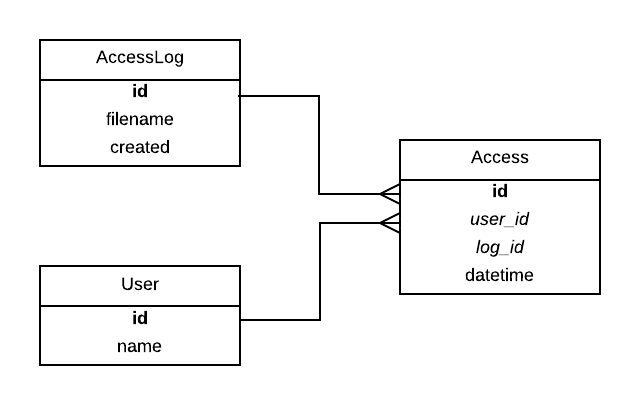
\includegraphics[scale=0.3]{media/diagrams/ERD.png}
    \end{figure}

    \subsection{Database Table Views}
        \subsubsection{Users}
            \begin{figure}[H]
                \caption{Screenshot of the Users table in the database.}
                \centering
                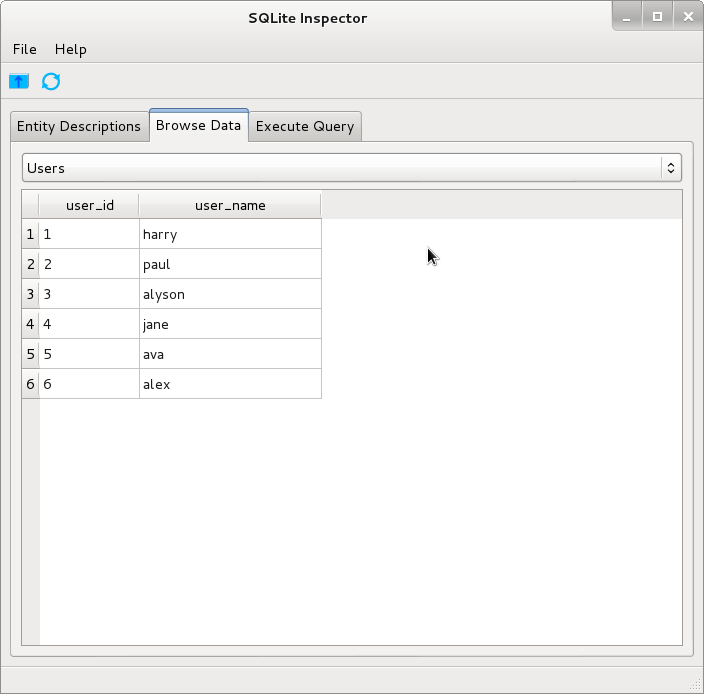
\includegraphics[scale=0.5]{media/screenshots/database_users.png}
            \end{figure}

        \subsubsection{Access}
            \begin{figure}[H]
                \caption{Screenshot of the Access table in the database.}
                \centering
                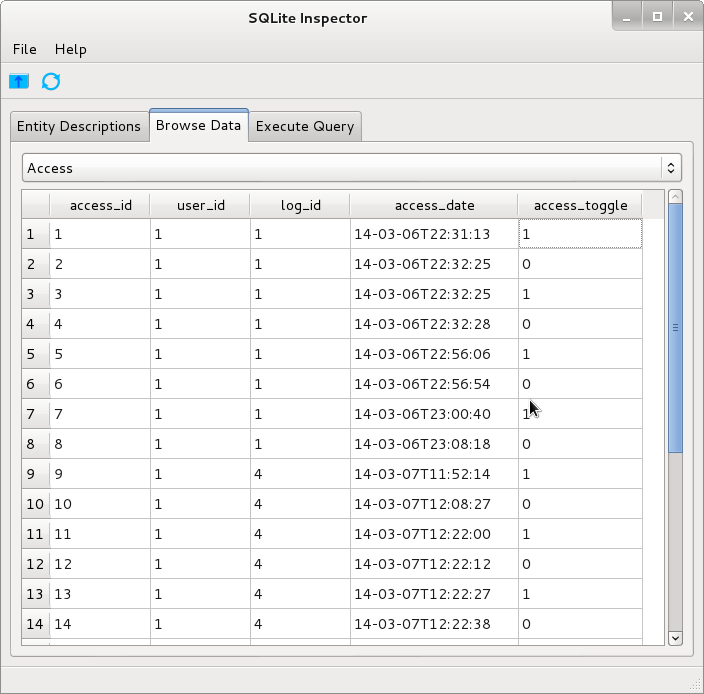
\includegraphics[scale=0.5]{media/screenshots/database_access.png}
            \end{figure}

        \subsubsection{Log}
            \begin{figure}[H]
                \caption{Screenshot of the Log table in the database.}
                \centering
                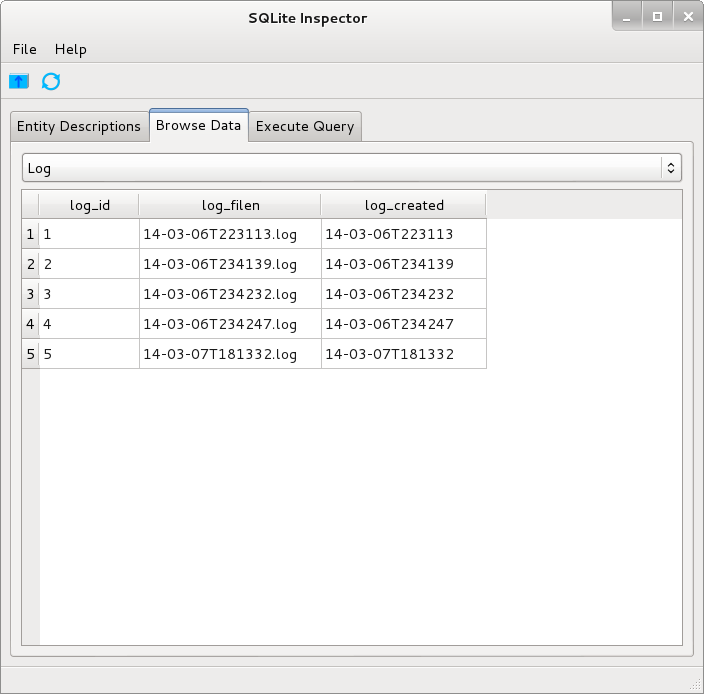
\includegraphics[scale=0.5]{media/screenshots/database_log.png}
            \end{figure}

        \newpage
        \subsection{Database SQL}

        \lstinputlisting[language=Python, 
                        firstline=32, 
                        lastline=56,
                        showstringspaces=false,
                        label={lst:createtables},
                        caption=Extract from sql\_interface.py]{code/server/sql_interface.py}
        Above, in Listing~\ref{lst:createtables}, you can see the function inside the `SQLInterface' class which creates the tables
        within the database. This function \textit{must} be ran before any other inside the class if the database
        hasn't been initialised before, otherwise an exception will be thrown saying either that the database 
        doesn't exist yet or the tables don't exist.

        The structure of this function has been coded with the `DRY' (`Don't Repeat Yourself') principle in mind;
        instead of running each SQL statement individually, the strings are in a list which can be iterated over.

    \subsection{SQL Queries}

    \begin{table}[H]
        \centering
        \begin{tabular}{|p{5cm}|p{8cm}|}
        \hline
        \textbf{Functionality}                                                                                                                   & \textbf{SQL Statement}                                                                                                                                          \\ \hline
        Creates a new User with the given user\_name.                                                                   & INSERT INTO Users(user\_name) values (?)                                         \\ \hline
        Delete a user with a given id.                                                                                  & DELETE FROM Users where user\_id = ?                                             \\ \hline
        Return all stored user\_name attributes in the Users table.                                                     & SELECT user\_name FROM Users                                                     \\ \hline
        Return all Users entities with the given user\_name.                                                            & SELECT * from Users WHERE user\_name = ?                                         \\ \hline
        Return the Users entity with the given user\_id.                                                                & SELECT user\_name FROM Users WHERE user\_id = ?                                  \\ \hline
        Create new Log entity with the given filename and created date.                                                 & INSERT INTO Log(log\_filen, log\_created) VALUES (?,?)                           \\ \hline
        Return the Log with the highest id number.                                                                      & SELECT * FROM Log WHERE log\_id=(SELECT MAX(log\_id) FROM Log)                   \\ \hline
        Create an entity in the Access table with the given attributes; user\_id, log\_id, access\_date and access\_toggle. & INSERT INTO Access(user\_id, log\_id, access\_date, access\_toggle) VALUES (?,?,?,?) \\ \hline
        Return all Access entities initiated with the given user\_id.                                                   & SELECT * FROM Access WHERE user\_id = ?                                          \\ \hline
        \end{tabular}
    \end{table}

\section{Testing}
    \subsection{Summary of Results}
        The results of testing, as shown in the `Testing' document, show that the code is for the most part empty of bugs. However, this
        has come at the cost of losing a few features, for example, the database browser doesn't include all of the features shown in the 
        design mock-ups of the user interface.

        Things that testing did show was that the system isn't easy to set up, luckily my intended client has an extensive knowledge of
        computer systems, he works as a CTO (Chief Technology Officer) and previously has had experience with programming languages such as
        C++ and Fortran 77.
    \subsection{Known Issues}
        Issues with this system are mostly security and set-up based, in it's current state it is very hard to keep the whole system running
        with each node up to date. 

        Some of the issues include:
        \begin{itemize}
            \item Server security
            \item Ease of Set-up
            \item System-wide Database updates
        \end{itemize}

\section{Code Explanations}
    \subsection{Difficult Sections}
        \subsubsection{Client}

        The below method, listing~\ref{lst:getcfg}, shows the method which is used to parse the configuration file for the client. First, on line 2,
        Python checks to see if `client.cfg' exists before running the rest of the code, if it doesn't, nothing will be parsed. On line 3 the function
        instantiates a `ConfigParser', which is a package which is included with Python. This is used as an abstraction of the configuration file, you
        read the file in on line 4. The last 3 lines are retrieving settings from the abstraction of the configuration file and setting them as attributes
        of the Client object. This is done so that these settings can be read from other functions without explicitly passing them.

        \begin{figure}[H]
        \lstinputlisting[language=Python, 
                        firstline=18, 
                        lastline=24,
                        label={lst:getcfg},
                        caption=get\_cfg method from section~\ref{sec:client.py}]{code/client/client.py}
        \end{figure}

        Listing~\ref{lst:clientstart} in section~\ref{sec:clientstructure} shows the start method of the Client class, on line 3 a infinite loop is started because we want to run this script
        as a daemon. Line 4 we retrieve a face from the camera and store the return value in the `face' variable, if a face wasn't detected the face variable
        will be equal to None, otherwise it will be an object from SimpleCV. Once a face is detected, line 7 will let the rest of the code run, so we can then
        check if it matches any of the stored faces in the client data folder. This works the same in that if it doesn't return a match result will equal None,
        so if it is a success it will fall through to line 10 where we send a packet to the server requesting an alarm toggle.

        \subsubsection{Server}

        \lstinputlisting[language=Python, 
                        firstline=25, 
                        lastline=41,
                        label={lst:linereceived},
                        caption=lineRecieved method from section~\ref{sec:server.py}]{code/server/server.py}

        The function in listing~\ref{lst:linereceived} is called as part of the Twisted package, when a string is received with the given delimiter this method is called. Here we are passed the
        data from the line which has been received, so we check if it is a valid request. The data is split by the white space so we can number the arguments, then
        we run through and check to see if these arguments are valid. If any of them are incorrect we will end the connection with the client and return them a string
        stating that it failed.

        \subsubsection{SQLInterface}

        \lstinputlisting[language=Python, 
                        firstline=112, 
                        lastline=123,
                        label={lst:logaccess},
                        caption=log\_access method from section~\ref{sec:sqlinterface.py}]{code/server/sql_interface.py}

        Listing~\ref{lst:logaccess} shows a very dense method from the SQLInterface class in section~\ref{sec:sqlinterface.py}, this is because it needs to handle two things;
        appending to a log file and adding to the database. The function fetches the user\_name from the database using the user\_id and generates a `datetime' string which is
        used to date both the database entry and log entry.
    \newpage
    \subsection{Self-created Algorithms}
        \subsubsection{Main Client Runtime}
        \begin{figure}[H]
        \caption{Client runtime as shown in \ref{sec:client.py} start function}
            \begin{algorithmic}
                \PRINT Starting loop...
                \WHILE{true}
                    \STATE $face\gets face\_detected()$
                    \IF{face}
                        \STATE $result\gets check\_face(face)$
                        \IF{result}
                            \STATE send\_auth(result)
                        \ENDIF
                    \ENDIF
                \ENDWHILE
            \end{algorithmic}
        \end{figure}


\section{Settings}
    \label{sec:settings}
    \subsection{Server}
    The server has it's settings contained in a `.cfg' file, which is placed in the same directory as `main.py',
    the system uses a Python object called `ConfigParser' which reads from this plain-text file and stores it in
    the object.
    \lstinputlisting[caption=server.cfg]{code/server/server.cfg}

    \subsection{Client}
    Listing 3 (below) is an example of a configuration file used by `client/client.py' which is shown in section~\ref{sec:client.py},
    this file contains key information which the client needs to connect and recognise faces. Under the `[network]' section
    on line 1 there are two settings, host and port, these are the variables used to point the client at the correct socket.
    The `port' is parsed as an integer and `host' as a string, the program then later concatenates the two together to create
    a server socket to connect to.

    On line 5 there is `[face \_settings]' which declares another set of settings within the configuration file, these are to do with
    the dependency `SimpleCV', which has a few system specific variables which need to be set by the administrator. The only setting
    under this section is `haar\_path' which points to the XML file containing a `Haar Cascade' reference file. Haar Cascade is the
    algorithm used to detect faces, it needs a file with previously collected face data to detect `general' faces
    \lstinputlisting[caption=client.cfg]{code/client/client.cfg}
\section{Acknowledgements}
    \subsection{Adam McNicol}
    The code I used to create the Database Browser was forked from the repository from github.com/MrAGi, I trimmed
    down the original code and edited things like the file browser to more suit my needs. Taking advantage of
    open source projects is a great way of saving time and learning from other peoples code. After seeing the code
    in use before, it seemed logical to just take that project and change it slightly to fit my project. The best
    thing about it was that it was already very well tested since the entire class had already been using it without
    any problems.

    \subsection{Code Listing Appendix}
        \subsubsection{client/client.py}
        \label{sec:client.py}
        \lstinputlisting{code/client/client.py}

        \subsubsection{server/main.py}
        \label{sec:main.py}
        \lstinputlisting{code/server/main.py}

        \subsubsection{server/server.py}
        \label{sec:server.py}
        \lstinputlisting{code/server/server.py}

        \subsubsection{server/sql\_interface.py}
        \label{sec:sqlinterface.py}
        \lstinputlisting{code/server/sql_interface.py}

        \subsubsection{db\_browser/db\_browser.pyw}
        \label{sec:dbbrowser.py}
        \lstinputlisting{code/db_browser/db_browser.pyw}

        \subsubsection{db\_browser/dialogs.py}
        \label{sec:dialogs.py}
        \lstinputlisting{code/db_browser/dialogs.py}

        \subsubsection{db\_browser/sqlite\_browse\_data.py}
        \label{sec:browsedata.py}
        \lstinputlisting{code/db_browser/sqlite_browse_data.py}

        \subsubsection{db\_browser/sqlite\_connection.py}
        \label{sec:connection.py}
        \lstinputlisting{code/db_browser/sqlite_connection.py}

\chapter{Evaluation}

\section{Customer Requirements}
	
	\subsection{General Objectives}
	
		\begin{itemize}
			\item Quick and easy to use method of user verification

			The program allows an easy method to toggle the alarm system successfully, all the user has
			to do is let the program scan their face, therefore this objective has been met. (Line 8 in Figure~\ref{lst:interview})


			\item Easy additional user set-up

			Setting up users with the client currently requires a function within the code to be ran,
			this is within the ability of the user but it is hard to call it `easy'. However, the database
			has a user interface which works correctly and adding users is very easy. (Line 10 in Figure~\ref{lst:interview})

			\item Communication with the server over the network

			The client correctly communicates back and forth with the server across a network. (Line 12 in Figure~\ref{lst:interview})
 
			\item Store users and access logs in a SQL database

			Users and logs are stored on the server in an SQL database, this database is only controlled
			by the system administrator. (Line 14 in Figure~\ref{lst:interview})
		\end{itemize}

	\subsection{Specific Objectives}

		\paragraph{User Verification}
			\begin{itemize}
				\item Ability to recognize faces

				The client successfully detects that a face is within the camera region, the `SimpleCV' package
				handles this very well. (Line 16 in Figure~\ref{lst:interview})

				\item Ability to tell different faces from others
				
				After matching the input with the saved files, the client can correctly match an input face with a
				user that has previously been stored on the file system. (Line 18 in Figure~\ref{lst:interview})

				\item Must be able to match a name to that face

				Images of the users are saved to the system with the file name as the user's name, this means there is
				no further processing to find the user's name after the input has been matched with a file. (Line 18 in Figure~\ref{lst:interview})
			\end{itemize}

		\paragraph{User Set-up}

			\begin{itemize}
				\item UI to edit each user or add users

				A database UI has been created for the server, however there is no user interface for the client, so I would
				say this objective is partially met.
				
				\item Power user tools

				The set-up allows raw access to the SQLite database, however, there are no power user tools coded into any of
				the system.
			\end{itemize}

		\paragraph{Network Communication}
		
			\begin{itemize}
				\item Access to local area network
                    
                    This objective has been met because the server and client sucessfully talk over the local area network
                    via sockets; the client sending commands to the server and recieving a response. (Line 12 in Figure~\ref{lst:interview})

				\item Receive commands and send commands
                    
                    As mentioned in the above objective, commands work from remote hosts. When the client asks the `status' of
                    alarms, the server responds. Similarly, the server responds when the client wants to register a user 
                    accessing the system. (Line 12 in Figure~\ref{lst:interview})

				\item Secure
                    
                    The system isn't secure enough for anyone with a certain amount of computing knowledge, as it is possible to
                    just send commands the the server without being authenticated, meaning that if anyone sends a packet to the
                    correct port on the server, they can turn the system on or off.

			\end{itemize}

		\paragraph{SQL Database}
		
			\begin{itemize}
				\item Table containing each user

					The Users table contains the user\_id and user\_name attributes.

				\item Access logs with a relationship to a user,

					Each access entry contains a user\_id foreign key which points to the user who triggered that event.

				\item Secure interface with communicating to the database.

					The system isn't secure, it has merely coded to be functional. This is because of a time limitation set by my teacher.

			\end{itemize}

	\subsection{Core Objectives}
		
		\begin{itemize}
			\item User verification via face recognition

				This objective has been met as shown in figure~\ref{lst:interview}.

			\item Interface with the server

				The client talks to the server via the local area network, therefore this objective has been met.

			\item Server to turn the alarms on and off

				This objective has been met as shown in figure~\ref{lst:interview} line 20.
		\end{itemize}

	\subsection{Other Objectives}
		
		\begin{itemize}
			\item Socket encryption

				Does not exist in the system.

			\item Control over what time slots people are allowed to turn alarms off

				Does not exist in the system.

			\item Ability to edit users from different computers

				Does not exist in the system.
		\end{itemize}




\section{Effectiveness}

	\subsection{Specific Objectives}

		\paragraph{User Verification}
			\begin{itemize}

				\item Must be able to match a name to that face

				This objective could have been carried out better, there is different way to implement user face recognition called HaarCascade. 
				Unfortunately, the time constraints didn't give me enough time to find a valid way of making adding a user to this method of face
				recognition easily. HaarCascade takes `training' this is hard to make into some form of user interface.


			\end{itemize}

		\paragraph{User Set-up}

			\begin{itemize}
				\item UI to edit each user or add users

				The database browser allows adding of users by a simple pop-up dialogue, the browser also enables an intuitive `double-click' method
				of editing existing entities in the table. (Line 22 in Figure~\ref{lst:interview})

			\end{itemize}


		\paragraph{SQL Database}
		
			\begin{itemize}
				\item Table containing each user

				The structure of the user database table was simple as it just gave each user an id which could be linked to the related entities.

			\end{itemize}

	\subsection{Core Objectives}
		
		\begin{itemize}
			\item User verification via face recognition

			The problem with this implementation is that it is easily spoofed, there is no `blink detection' to combat the imitation of the user. 

			\item Interface with the server

			The clients commands to the server aren't very effective because there is no source authentication, an ideal fix to this would be some form of
			initial authentication phase so that the server has the client's unique identifier.
		\end{itemize}


\section{Learnability}
	The interface of the database browser is similar to other software's user interfaces, this makes it easy to understand. The client expressed this in
	line 22 figure~\ref{lst:interview}.

	\begin{figure}
		\begin{center}
		\caption{A screenshot of the database browser}
		\label{fig:db_browser}
		\includegraphics[scale=0.5]{media/screenshots/db_browser_eg.png}
		\end{center}
	\end{figure}

	Above, in figure~\ref{fig:db_browser}, you can see how the elements match common software interfaces. For example, the `menubar' contains a `file'
	menu which contains things like `New' and `Open'. The table is also similar to that of excel, you can click to edit. 


\section{Maintainability}

	The code in this project is very modular, the different sections of it have been abstracted into classes, not only this but the functions inside these
	classes are mostly easy to understand since each function has a simple task. However, the code lacks comments in it's current state, so at the individual
	line level, it may require some more research as to the modules referenced in the code. The code only uses local variables, this means understanding where
	data comes from is a lot easier to that of a program which takes use of global variables.

\section{Suggestions for Improvement}

	\begin{itemize}
		\item Improved accuracy of face recognition

			The issue with this is in it's current state it takes way too long for the system to take a picture which is sufficient to match with the stored
			images of the user, this is vital because it is detrimental to the main objective of the system; to make the user authentication easier.

		\item Secure sockets

			This is a less important issue as the local network will actually already have protection from the fact you need to be connected to it in the first place,
			however this isn't an assumption I would like to make. The data sent to and from the client and server \textit{should} be encrypted.

		\item Authenticated clients 

			This is linked to the system being secure, without any kind of authentication anybody can send data to the server and get a response or trigger an event, this
			is highly undesirable.

		\item Synced databases

			Keeping all of the clients and server updated with the same version of database is something which would require a \textit{lot} of work from the system administrator,
			this currently is an unacceptable amount. Ideally, whenever a client is made on an \textit{authenticated} device, it'd tell the server and the server would inform the
			rest of the clients.

	\end{itemize}	

\section{End User Evidence Appendix}

	\subsection{Interview}

		\begin{figure}
			\caption{Feedback interview}
			\label{lst:interview}
			\lstinputlisting{media/eval_interview.log}
			\includegraphics[scale=0.7]{media/pmilnesignature.png}
		\end{figure}
		
\newpage
\chapter{User Manual}

\section{Introduction}
    This documentation has been written in mind with the user having a standard knowledge with Linux and the operating system being a
    distribution of Ubuntu which uses the aptitude package manager.

    The intended audience of this system is a normal household, in this case it is Paul Milne's household. Paul himself is very experienced
    in computing, however the rest of the household have an average IT knowledge.

    The purpose of the system is to provide an easy method to interface with the alarms; to turn them on and off. 

\section{Installation}

    \subsection{Prerequisites}

        \subsubsection{Hardware}

            \begin{itemize}
                \item Computer network within intended house
                \item Computer with camera attached for client
            \end{itemize}

        \subsubsection{Software}

            \begin{itemize}
                \item Python 2.7 - \textit{all}
                \item Qt UI Library - \textit{db\_browser}
                \item SimpleCV - \textit{client}
                \item svgwrite - \textit{client}
            \end{itemize}

    \subsection{System Installation}
        If you do not already have the files they are available for download at: \url{https://github.com/harrymilne/face_recognition_a2}.
        This repository has two root folders, `code' and `docs', Python files for the running of the client and server are under code.
        Once you are in the code directory this then has 3 folders, `client', `db\_browser' and `server', the `server' and `db\_browser'
        folders need to be on the same computer, whereas the client needs to be placed on a computer with access to a network capable of
        connecting to the computer which has the `server' and `db\_browser' folders on. 

    \subsubsection{Client}
        The client software must be installed anywhere you want end-users to be able to control the system, the code can be ran on a 
        raspberry pi or on a `normal computer'. 
        The client (face recognition) requires a Python package called SimpleCV, to install this you must first 
        download the `superpack' from simplecv.org/download (shown in figure~\ref{fig:simplecv}).  This installs all of the dependencies 
        you need for the client program.

        \begin{figure}[H]
            \centering
            \caption{A screenshot of the SimpleCV website where it is possible to download the `superpack'.}
            \label{fig:simplecv}
                \includegraphics[scale=0.7]{media/screenshots/manual/simplecv_download.png}
        \end{figure}

        \paragraph{Linux}
        \begin{enumerate}
            \item Install required system packages for your system using aptitude with the command given below.

            \textit{sudo apt-get install ipython python-opencv python-scipy python-numpy python-pygame python-setuptools python-pip}

            \item Install required packages for Python.

            \textit{sudo pip install SimpleCV svgwrite}

            \item Check the installation was successful. As shown in figure~\ref{fig:simplecvcheck}, this shows that the command ran
            without error.

            \textit{python -c `import SimpleCV'}
            \begin{figure}[H]
                \centering
                \caption{Example of command running without failure.}
                \label{fig:simplecvcheck}
                    \includegraphics[scale=0.6]{media/screenshots/manual/pychecksimplecv.png}
            \end{figure}

            \item Check that the camera is being detected by SimpleCV by running Python, importing SimpleCV and instantiating a 
            Camera object without error. As shown in figure~\ref{fig:cameracheck}.

            \begin{figure}[H]
                \centering
                \caption{Instantiating a Camera object.}
                \label{fig:cameracheck}
                    \includegraphics[scale=0.6]{media/screenshots/manual/pycheckcamera.png}
            \end{figure}

            \item Add required users by entering the client directory at `code/client' and run the following: \newline
            \textit{python client.py adduser $<$username$>$} \newline
            This should create the directories and take a picture of your face when it is in the frame of the camera. It will have
            created a user when there is a `$<$username$>$.jpg' file in the data folder.

        \end{enumerate}
        \textit{Instructions on how to install SimpleCV on other operating systems can be found here: \url{https://github.com/sightmachine/SimpleCV/blob/master/README.markdown}.}

        \paragraph{Settings}\mbox{}\\
            The files included with the downloaded repository will include an example configuration file called `client.cfg'. As shown
            below in figure~\ref{lst:clientcfg}, this must but set to use values that suite your system needs. To find the `haar\_cascade'
            path you must find where your Python installation resides and check `dist-packages' for the `SimpleCV' folder, then it should
            be under `Features/HaarCascades' as of version 1.3. \newline
            \textit{host} should be the local IP address of the server. \newline
            \textit{port} should be the port the server is running on, which is also defined in the `server.cfg'.

            \begin{figure}[H]
                \centering
                \caption{Example client configuration included in code repository.}
                \label{lst:clientcfg}
                    \lstinputlisting{code/client/client.cfg}
            \end{figure}

    \subsubsection{Server}
        The server needs to be installed on a computer that will be up all of the time, this is because people need to be able to access
        the alarm system any time of the day.

        \paragraph{Linux}

        \begin{enumerate}
            \item Install required system packages using aptitude with the command given below.

            \textit{sudo apt-get install python-setuptools python-pip}

            \item Install Twisted Python package.

            \textit{sudo pip install twisted}

            \item Check the Twisted installation, as shown below in figure~\ref{fig:twistedcheck}.

            \textit{python -c `import twisted'}
            \begin{figure}[H]
                \centering
                \caption{Example of command running without failure.}
                \label{fig:twistedcheck}
                    \includegraphics[scale=0.6]{media/screenshots/manual/pychecktwisted.png}
            \end{figure}
        \end{enumerate}

        \paragraph{Settings}\mbox{}\\
        The servers settings are all stored in a file called `server.cfg', these are shown in figure~\ref{lst:servercfg}. It isn't
        necessary to change these, only unless something is already running on the port given by default.

        \begin{figure}[H]
            \centering
            \caption{Example client configuration included in code repository.}
            \label{lst:servercfg}
                \lstinputlisting{code/server/server.cfg}
        \end{figure}

    \subsection{Database Browser}
        \paragraph{Linux}\mbox{}\\
        \begin{enumerate}
            \item Install system and Python packages using aptitude with the command given below.

            \textit{sudo apt-get install libqt4-sql-sqlite python-qt4 python-qt4-sql}

            \item Once these packages have finished installing, try and run the `db\_browser.pyw' file with `\textit{python db\_browser.pyw}'.
            A window should pop-up as shown in figure~\ref{fig:dbbrowserrun}.

            \begin{figure}[H]
                \centering
                \caption{Example of the Database Browser running.}
                \label{fig:dbbrowserrun}
                    \includegraphics[scale=0.6]{media/screenshots/manual/dbbrowserrun.png}
            \end{figure}
        \end{enumerate}

\section{Tutorial}

    \subsection{Introduction}
        I will break down how to use each part of the system in the sections below, each sub-section will include one feature of
        the system explained with detailed text instructions and annotated diagrams to assist you in running the system to its full extent.

    \subsection{Assumptions}
        Assumptions have been made around the proficiency of the user, these include knowing how to start a Python script and having a lot of
        experience previously working with computers.

    \subsection{How to start the server}
        To run the server you must be in the `code/server/' directory and run `\textit{python main.py}'. In figure~\ref{fig:serverrun} you can 
        see the server successfully running.
        \begin{figure}[H]
            \centering
            \caption{Example of the server running.}
            \label{fig:serverrun}
                \includegraphics[scale=0.6]{media/screenshots/manual/serverrun.png}
        \end{figure}


    \subsection{Running the server as a daemon}
        Running the server as a daemon requires a shell window manager, this keeps a process running which will otherwise be quit when the user
        logs out of the SSH protocol. An example of a suitable window manager is `screen', to install this on Linux you can run 
        `\textit{sudo apt-get install screen}', once installed correctly you can follow the steps below to run the server as a daemon.
        \begin{enumerate}
            \item Run `\textit{screen -S face-server}'.

            This'll spawn a `screen' in which will persist even when the user has logged out of the shell, however your shell will look no different
            apart from being cleared from previous text. To exit this screen you can type `\textit{exit}' while attached to the screen which will terminate
            it. Otherwise, you can hold the \textit{CTRL+A+D} keyboard combination; this'll detach you from the screen, once detached you can reattach to 
            the screen by typing `\textit{screen -r face-server}'.

            \begin{figure}[H]
                \centering
                \caption{Example of `screen' commands.}
                \label{fig:screen}
                    \includegraphics[scale=0.6]{media/screenshots/manual/screen.png}
            \end{figure}

            \item While in the `server' directory of the repository run `\textit{python main.py}', and you can then detach from this by using the steps
            explained in step 1.

        \end{enumerate}

    \subsection{How to start the client}
        To run the client you must be in the `code/client/' directory and run `\textit{python client.py}'. In figure~\ref{fig:clientrun} you can 
        see the client successfully running.
        \begin{figure}[H]
            \centering
            \caption{Example of the client running.}
            \label{fig:clientrun}
                \includegraphics[scale=0.6]{media/screenshots/manual/clientrun.png}
        \end{figure}


    \subsection{How to start the database browser}
        To run the database browser you must be in the `code/db\_browser/' directory and run `\textit{python db\_browser.pyw}'. In figure~\ref{fig:dbbrowserrun} you can 
        see the database browser successfully running.

    \subsection{How do I create a new user?}
        This requires actions on both the server and client, firstly the user must be added to the server database so that the client request 
        succeeds when prompted. This requires running the `db\_browser' and adding a user via the provided user interface, in figure~\ref{fig:dbadduser}
        you can see the `File' menu being opened and a new user dialogue popping up.

        \begin{figure}[H]
            \centering
            \caption{Example of new user dialog.}
            \label{fig:dbadduser}
                \includegraphics[scale=0.7]{media/screenshots/manual/dbadduser.png}
        \end{figure}

        Secondly, a user must be added to the client, this can be done by facing the user in front of the camera and running `\textit{python client.py adduser $<$name$>$}',
        or images with the face of the user cropped can be added to the `client/data/usr' folder with $<$name$>$.jpg naming convention.
    \newpage
    \subsection{How do I start a new log file?}
        To create a new log you simply select File $>$ New $>$ Log File, from the Database Browser, as shown in figure~\ref{fig:dbaddlog}.

        \begin{figure}[H]
            \centering
            \caption{File $>$ New Menu}
            \label{fig:dbaddlog}
                \includegraphics[scale=0.5]{media/screenshots/manual/dbaddlog.png}
        \end{figure}        


\section{Errors}
    \subsection{SimpleCV/Camera related}
        \begin{figure}[H]
            \centering
            \caption{Example of a camera not found error}
            \label{fig:camera404}
                \includegraphics[scale=0.5]{media/screenshots/manual/camera404.png}
        \end{figure} 
        This error will occur to the client when a camera has not been detected by SimpleCV, to fix this you can follow the steps below:
        \begin{enumerate}
            \item Check the camera is connected to the client computer
            \item Check the camera's drivers are installed
            \item Try a different USB port
        \end{enumerate}



    \subsection{Network related}
        \begin{figure}[H]
            \centering
            \caption{Example of a network error}
            \label{fig:networkcrash}
                \includegraphics[scale=0.5]{media/screenshots/manual/networkcrash.png}
        \end{figure} 
        This error will occur to the client file when it cannot reach the server, this is because when the client is initially started the 
        server is queried by the client and when the client cannot connect to the given port, this error is raised. To fix this you either
        need to:
        \begin{enumerate}
            \item Check the server is running, if not start it
            \item Check the client is pointed towards the right socket
            \item Check the client or server have access to the local area network
        \end{enumerate}

    \subsection{Database}
        \begin{figure}[H]
        \centering
        \caption{Example of a database error}
        \label{fig:db404}
            \includegraphics[scale=0.4]{media/screenshots/manual/db404.png}
    \end{figure} 
    This error will occur to the server when the database has not been initialised; this means that the SQLite database probably doesn't exist.
    To fix this you should run `python sql\_interface.py' to initialise the database, if this doesn't work then you can check the following:
    \begin{enumerate}
        \item Check the database is located in the same folder as `server.py'
        \item Check the database file hasn't been renamed
    \end{enumerate}
\newpage
\section{System Recovery}
    \subsection{Backing up data}
        \subsubsection{Client}
            \begin{enumerate}
                \item Compress the `data' folder within the client folder.
                \begin{center}
                \includegraphics[scale=0.4]{media/screenshots/manual/compressclientdata.png}
                \end{center}
                \item Store this compressed copy of the folder on a different medium, such as USB
                \begin{center}
                \includegraphics[scale=0.4]{media/screenshots/manual/clientstoredusb.png}
                \end{center}
            \end{enumerate}
            All of the sensitive data stored on the client are now backed up in a different medium or folder.
        \newpage
        \subsubsection{Server}
            \begin{enumerate}
                \item Compress the `logs' folder within the client folder.
                \begin{center}
                \includegraphics[scale=0.4]{media/screenshots/manual/compressserverdata.png}
                \end{center}
                \item Store this compressed copy of the folder and the `access.sqlite3' file on a different medium, such as USB
                \begin{center}
                \includegraphics[scale=0.4]{media/screenshots/manual/serverstoredusb.png}
                \end{center}
            \end{enumerate}
            All of the sensitive data stored on the server are now backed up in a different medium or folder.

    \subsection{Restoring data}
        \subsubsection{Client}
            \begin{enumerate}
                \item Decompress the backed up `data' zip.
                \begin{center}
                \includegraphics[scale=0.7]{media/screenshots/manual/decompressedclient.png}
                \end{center}
                \item Delete the pre-existing data folder, if it exists, in the client folder.
                \begin{center}
                \includegraphics[scale=0.7]{media/screenshots/manual/deleteclientdata.png}
                \end{center}
                \item Move this back up uncompressed data folder back into the client folder.
                \begin{center}
                \includegraphics[scale=0.6]{media/screenshots/manual/restoreclient.png}
                \end{center}
            \end{enumerate}
            The client will now be restored to the latest back up.
        \newpage
        \subsubsection{Server}
            \begin{enumerate}
                \item Overwrite the existing `access.sqlite3' with the backed up version.
                \begin{center}
                \includegraphics[scale=0.5]{media/screenshots/manual/serveroverwritedb.png}
                \end{center}
                \item Delete the pre-existing `logs' folder, if it exists, in the server folder.
                \begin{center}
                \includegraphics[scale=0.7]{media/screenshots/manual/serverlogdelete.png}
                \end{center}
                \item Decompress the backed up `logs' folder.

                \item Move this back up uncompressed logs folder back into the server folder.
                \begin{center}
                \includegraphics[scale=0.6]{media/screenshots/manual/serverlogmove.png}
                \end{center}
            \end{enumerate}


\end{document}
